\chapter{Reinforcement Learning}
The robot controls its motors using artificial neural networks (ANN) and the deep deterministic policy gradient (DDPG) algorithm, developed by Lillicrap et al.\ \cite{lillicrap_2016}. The system runs in Python 3 \cite{python3}, leaning heavily on the TensorFlow library with GPU support \cite{tensorflow} for artificial neural network instantiation, updating, and saving. After training, the system actuates each of the four drive motors to move the robot to a desired position and orientation in the Roborodentia field while minimizing the velocity and effort applied (i.e. energy spent). Two different approaches are implemented to compare DDPG performance with three separate single-output actors versus a single multiple-output actor. Before delving into the implementation and results, the following sections briefly cover reinforcement learning (RL) techniques that form the foundation of DDPG. It is worth noting that Sutton's introductory book on RL provides excellent background on many of the following algorithms and more \cite{sutton_2017}. 

\section{Reinforcement Learning Background}
Reinforcement learning (RL) is a subset of machine learning that aims to solve control and action selection problems rather than to perform classification or data clustering. In other words, the concern lies in determining which actions an actor should take in an environment to receive the greatest reward. Most reinforcement learning problems involve six main elements: an actor, the environment, rewards, a policy, a value function, and sometimes a model. An actor (sometimes called an agent) takes actions in an environment which returns a state and reward, illustrated in Figure \ref{fig:actor_env_loop}. The full state encompasses all the parameters of the environment and actor such as position, velocity, color, size, or any other measurable quantity; although the term ``state'' in this context refers to the subset of parameters observed by the actor. The actor's primary goal is to maximize the accumulated reward received from the environment. A policy determines which actions the actor takes given the current state. The value function indicates the long-term reward expected from a state and is defined for all possible states. To compare reward with value, even if a state only has a small immediate reward, it may possess high value since it leads to future high reward states. Finally, some algorithms involve a model of the environment, allowing prediction of the next state from the current state and action. Table \ref{tab:rl_defs} summarizes some common terms and definitions used in the reinforcement learning literature.
\begin{figure}[H]   % [h] means here
	\centering 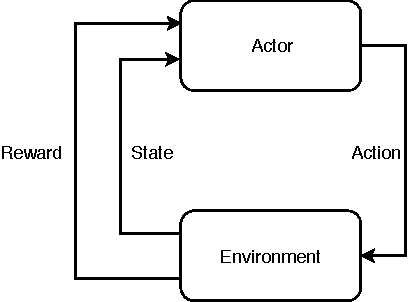
\includegraphics[width=3in, height=3.85in, keepaspectratio]{figures/actor_env_loop.pdf}
	\caption{Actor-Environment Feedback Loop}\label{fig:actor_env_loop}
\end{figure}
\LTXtable{\textwidth}{tables/tab_rl_defs.tex}

To better conceptualize these terms, consider a game of tic-tac-toe as shown in Figure \ref{fig:tictactoe}. The \textbf{environment} is the game itself, including the rules and game board. The two \textbf{actors} (players) sequentially take the \textbf{action} of placing marks in the boxes. The actions are encoded into some numeric form as defined by the designer. For example, $a=0$ might represent putting an X in the top left corner while $a=9$ might mean an X in the bottom right corner. Winning the game would grant a good \textbf{reward} while tying or losing might yield a bad reward. The reward could also come turn-by-turn instead of at the end of the game. Lining up marks for a win might produce a good reward while letting the opponent set a trap might be bad. The designer could even assign reward magnitudes to weight the significance of each state. Note that the descriptors ``good'' and ``bad'' are deliberately vague as numerous valid implementations of the reward exist. Conceptually, the reward allows the actor to differentiate between desirable and undesirable actions and states. No single ``correct'' reward implementation exists, but one should be chosen to reflect the desired policy. Each of the nine spaces can take one of three values (blank, X, or O) so the game has $3^9=19,683$ possible \textbf{states} (although some states are not achievable as the game would end once a player gets three in a row). Like the action, the rewards and states are represented numerically.
\begin{figure}[H]   % [h] means here
	\centering 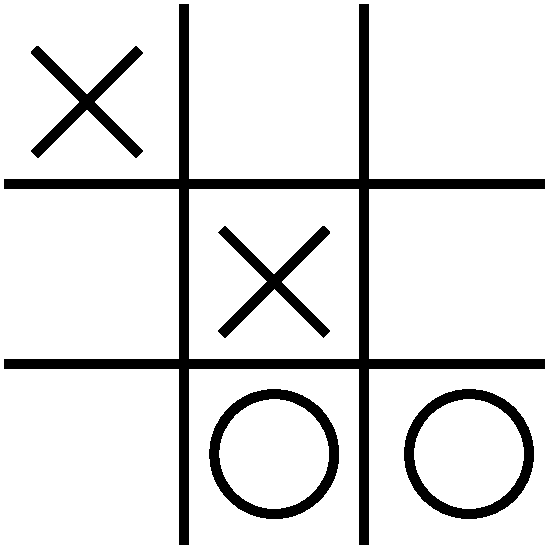
\includegraphics[width=2in, height=3.85in, keepaspectratio]{figures/tictactoe.pdf}
	\caption{A Game of Tic Tac Toe}\label{fig:tictactoe}
\end{figure}

\subsection{Long-Term Reward}
Actors strive to maximize the long-term discounted reward, $G_t$, where the subscript $t$ denotes the time step \cite{sutton_2017}. As mentioned previously, reward reflects the actor's policy. For example, the goal of tic tac toe is to win which, to the actor, is equivalent to taking actions that lead to states that lead to good rewards. In RL problems with a definitive end (denoted by $t=T$) such as a game of chess, $G_t$ is finite and can be calculated simply as the sum of all future rewards as shown in Equation \ref{eq:Gt_simple}. Additionally, the long-term aspect accounts for problems with intermediate rewards at each step. In chess, constantly trying to capture enemy pieces might yield some immediate good reward but may not actually be the best strategy for long-term success (i.e. winning the game).
\begin{equation}
	\label{eq:Gt_simple}
	G_t=R_{t+1}+R_{t+2}+\dots + R_{T}=\sum_{k=t}^{T-1} R_{k+1}
\end{equation}

However, continuous problems, such as maintaining the temperature of a refrigerator, have no maximum time step and therefore, a possibly infinite $G_t$. Shown in Equation \ref{eq:Gt_discount}, the introduction of a discount factor, $\gamma$, makes such a situation manageable. The discount factor weights the worth of future rewards exponentially by their distance into the future and ranges from 0--1 where 0 completely devalues future rewards while a discount factor of 1 weights all future rewards equally. In practice, the discount factor is less than 1 in order to allow $G_t$ to converge \cite{sutton_2017}. The discount factor can be considered a knob that sets the algorithm's outlook between myopic (short-sighted, only values immediate rewards) and far-sighted (willing to sacrifice immediate reward for greater long-term returns).
\begin{equation}
\label{eq:Gt_discount}
	G_t=R_{t+1}+\gamma R_{t+2}+\gamma^2 R_{t+3} + \dots = \sum_{k=0}^{\infty} \gamma^k R_{t+k+1}
\end{equation}

\subsection{Value Functions}
The \textbf{value} function $V_\pi(s)$ is the expected long-term reward $G_t$ as a function of the state $s$ under a certain policy $\pi$, written out in Equation \ref{eq:value_func}. The $\mathbb{E}_\pi$ operator evaluates the expected value provided the actor continues to take actions following policy $\pi$.
\begin{equation}
	\label{eq:value_func}
	V_\pi(s)=\mathbb{E}_\pi [G_t | s]
\end{equation}

Related but slightly different, the \textbf{Q-function} or \textbf{action-value} function $	Q_\pi(s,a)$ is the expected long-term reward $G_t$ as a function of the state $s$ \textbf{and action} $a$ under a certain policy $\pi$, shown in Equation \ref{eq:q_func}. The important distinction from the value function is dependency on the action. While the value function describes the expected long-term reward from being in a particular state and continuing to follow actions under the policy $\pi$, the Q-function returns the expected long-term reward from being in a particular state, taking a specific action, then continuing to follow actions under the policy $\pi$. Since the Q-function uses three variables ($s$, $a$, and $Q$), it can be plotted in three dimensions as in Figure \ref{fig:q_ex_plot}. Note that this is arbitrary plot for demonstration purposes more than representing actual Q-values for any particular environment. 

Considering tic tac toe, if $s=0$ represents the starting, i.e. blank, state of the game, the red slice of Figure \ref{fig:q_ex_plot} would represent the Q-values or expected long-term reward for each of the nine possible starting actions. Likewise, every slice would represent Q-values for the various actions taken in other game states, and the plot would have as many slices as there exist game states. Again, note that this is only an example and not the actual plot of tic tac toe's Q-function; it would use discrete points rather than the continuous function shown. The Q-function is defined for all possible states and actions so tic tac toe contains $19,683 \text{ states} \cdot 9 \text{ actions} = 177,147$ discrete Q-values. Notice that the Q-function is non-obvious, highly non-linear, and may be continuous or discrete depending on the specific problem.
\begin{equation}
	\label{eq:q_func}
	Q_\pi(s,a)=\mathbb{E}_\pi [G_t |s,a]
\end{equation}
\begin{figure}[H]   % [h] means here
	\centering 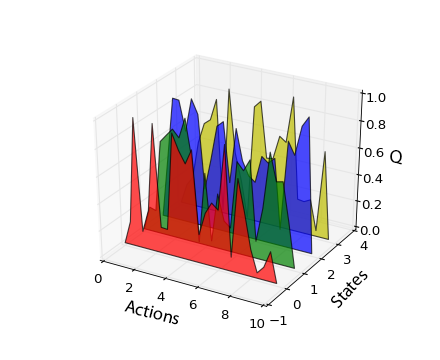
\includegraphics[width=4in, height=3.85in, keepaspectratio]{figures/q_ex_plot.png}
	\caption{3D Q-Function Example}\label{fig:q_ex_plot}
\end{figure}

\subsection{Policies}
Various policies exist but some of the most common include optimal, greedy, $\epsilon$-greedy, and random. The optimal policy $\pi_*$, by definition, produces greater or equal value for every possible state than any other policy $\pi$, expressed in Equation \ref{eq:optimalpol}, where $v_{\pi_*}$ represents the value function of the optimal policy, $v_{\pi}$ is the value function of any other policy $\pi$, and $\mathcal{S}$ is the set of all possible states. Ideally, the actor would eventually discover the optimal policy, but in reality, training always produces a sub-optimal policy except for the simplest of environments. 
\begin{equation}
	\label{eq:optimalpol}
v_{\pi_*}(s) \geq v_{\pi}(s), \forall s \in \mathcal{S}
\end{equation}
An actor under the random policy always takes random actions while the greedy policy directs the actor to take the action with the highest value or Q-value depending on implementation. Although greediness does lead the actor to take actions that it believes maximize the reward, it may also cause the actor to get stuck following a suboptimal policy. For example, if a greedy actor is learning tic tac toe, it may discover that putting an X in the middle of the top row as the first move led it to win. Being greedy, it will keep putting the mark there since it sometimes leads to a reward. However, if the actor would stop being greedy and try something new, it would eventually discover that putting the first mark in a corner leads to victory more often. In other words, an actor following a greedy policy may not sufficiently explore the environment, i.e. try new things to discover better actions or states which lead to even greater reward. To allow a balance between exploration (discovering better rewards) and exploitation (obtaining as much reward as it can), the $\epsilon$-greedy policy tells an actor to pick the greedy action with probability $1-\epsilon$ and a random action with probability $\epsilon$ where $\epsilon$ ranges between 0 and 1. 


\section{Reinforcement Learning Algorithms}
Many reinforcement learning algorithms have been applied to action selection and control problems including Q-Learning, State-Action-Reward-State-Action (SARSA), deep Q-network (DQN), policy gradients (PG), deep policy gradients (DPG), and deep deterministic policy gradients (DDPG), among others \cite{sutton_2017}\cite{sutton_policygrad}\cite{silver_2017}\cite{silver_lever_heess_degris_wierstra_riedmiller}\cite{lillicrap_2016}. Note that these methods differ from evolutionary algorithms in that they actively learn as they interact with the environment. Instead, evolutionary techniques evaluate the performance of individual actors in a population by determining how much reward each produces while operating in the environment, take the best performers, mutate them slightly to produce new behaviors, and repeat until a good policy emerges. The process is highly reminiscent of natural selection while the algorithms to be discussed are more akin to a child learning to walk \cite{natural_selection}.

RL algorithms can be classified by their use of models (model-based vs.\ model-free) and actor policy (on-policy vs.\ off-policy) \cite{sutton_2017}. Model-based strategies first develop a model of the environment and then use a planning algorithm along with the model to create a controller, while model-free algorithms forgo the model entirely. On-policy strategies learn the policy followed by the actor while off-policy techniques learn a policy different from the one followed by the actor. For example, in Q-learning, the Q-function updates its weights based on the next state and the greedy action (which is not actually executed) even if the actor is following the random policy \cite{sutton_2017}. The greedy action is determined by searching the Q-function in the next state for the action producing the highest Q-value, further explained in the Q-Learning section.

\subsection{Q-Learning}
Q-Learning is an off-model, off-policy algorithm that estimates the Q-function of the environment \cite{sutton_2017}. The Q-function represents the ``quality'' of every possible action in every possible state. Given a particular state, the Q-function returns the quality, i.e.\ predicted goodness, of each possible action the player could take. Therefore, the optimal action to take is simply the one with the highest Q-value. 

Clearly, the Q-function always exists but not necessarily in an analytic or obvious form. So-called tabular Q-learning methods use a 2-D matrix to represent the Q-function with rows for all possible states and columns for all possible actions \cite{mccullock}. The table is initialized with guesses (possibly randomly or with all elements set to 0) and iteratively updated to produce an approximation closer and closer to the true Q-function $Q^*$ using the Bellman equation presented in Equation \ref{eq:bellman}. The equation states that the expected long-term reward Q for state $s$ and action $a$ is equal to the reward received from being in state $s$ plus the discounted ($\gamma$) maximum Q of the next state $s'$. In simpler terms, the expected long-term reward is the current state's reward plus the best reward obtainable in the next state (weighted by $\gamma$). For clarity, the $\text{max}_{a'}(\cdot)$ operator chooses $a'$ to maximize its argument $(\cdot)$ so $\text{max}_{a'}(Q(s',a'))$ means the maximum Q of the next state $s'$ irrespective of the action $a'$. The proof that the Bellman equation does allow iterative Q-value calculation is beyond the scope of this thesis, but Sutton's book, \textit{Reinforcement Learning: An Introduction}, provides further explanation \cite{sutton_2017}.
\begin{equation}
	\label{eq:bellman}
	Q(s,a)=R(s) + \gamma (\text{max}_{a'}(Q(s',a')))
\end{equation}

To improve convergence, i.e. when the estimated Q-function approaches the optimal $Q^*$, Equation \ref{eq:bellman} is modified to include the learning rate $\alpha$, ranging between 0 and 1, which reduces the change in the Q-function with each iteration, shown in Equation \ref{eq:bellman_alpha}. The pseudocode for Q-learning presented by Sutton is reproduced in Table \ref{list:qlearning_pseudo} with permission. Some environments, like chess, eventually terminate (at the end of the game) while others, such as maintaining a refrigerator's temperature, may never actually terminate.
\begin{equation}
	\label{eq:bellman_alpha}
	Q(s,a)=(1-\alpha)Q(s,a) + \alpha[R(s) + \gamma (\text{max}_{a'}(Q(s',a')))]
\end{equation}
\begin{clisting}[caption={Q-Learning Pseudocode},label={list:qlearning_pseudo}]
Initialize Q(s,a) arbitrarily. 
Repeat for each episode: 
	Initialize s
	Repeat for each step of episode:
		Choose a from s using policy derived from Q (e.g., epsilon-greedy)
		Take action a, observe r, s'
		Q(s,a) = (1 - alpha) * Q(s,a) + alpha * [r + gamma * max_a(Q(s',a'))]
		s = s';
	until s is terminal 
\end{clisting}

Notice the algorithm recursively updates the Q-value, $Q(s,a)$, from the Q-value of the next state and greedy policy action, $\text{max}_{a'}Q(s',a')$, regardless of the policy and action taken by the actor. This characteristic makes Q-learning an off-policy algorithm. The Q-value for a particular state and action only updates when the actor visits said state and action so the actor must still explore (i.e.\ not always take greedy actions) for Q-learning to converge. Figure \ref{fig:q_learning_ex} illustrates an example of one step of recursive Q-function update using the tic tac toe. 
\begin{figure}   % [h] means here
	\centering 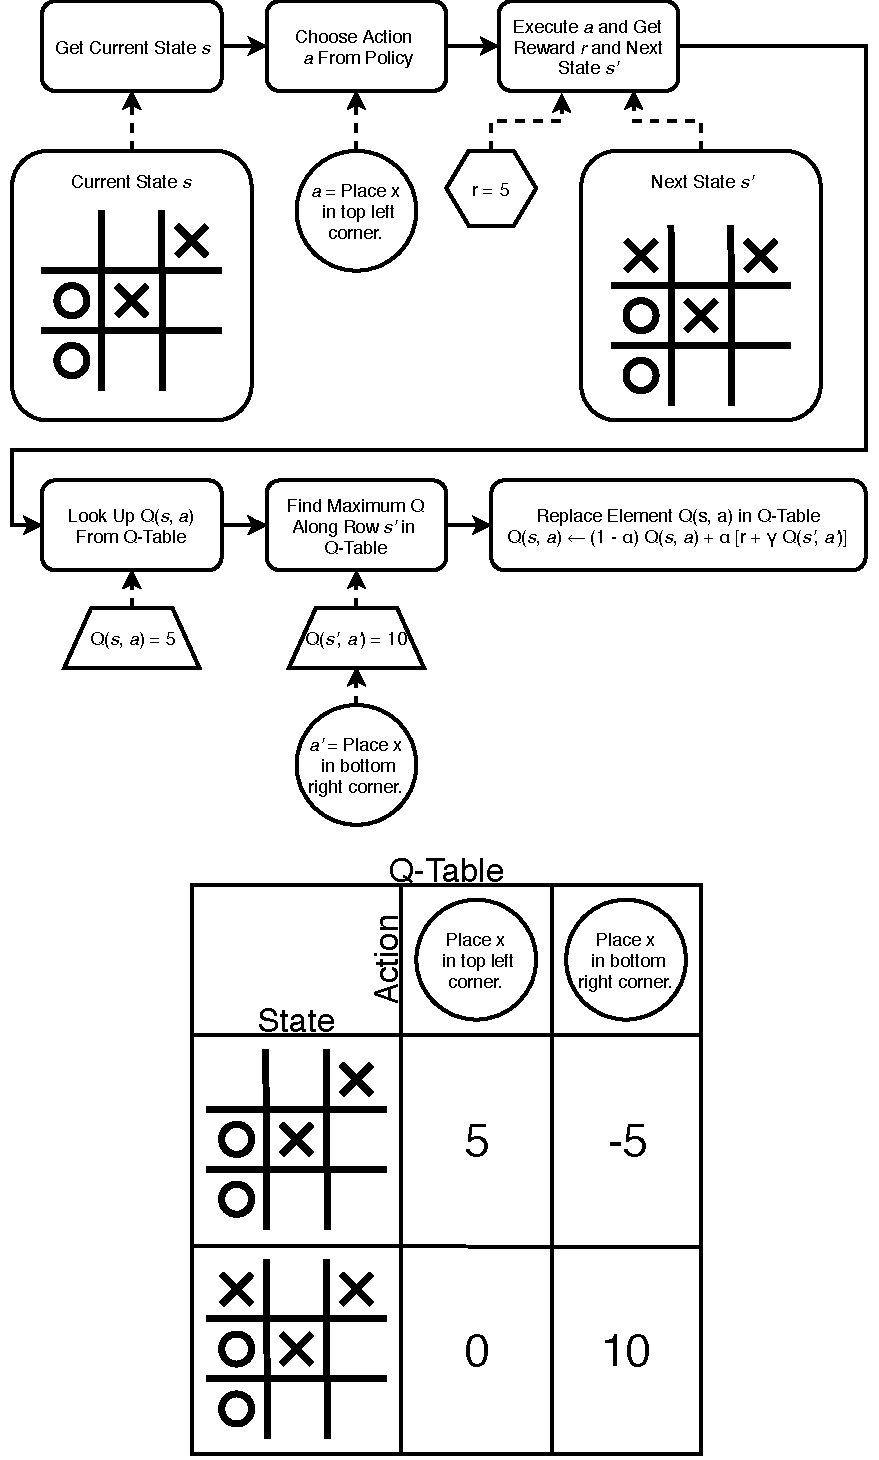
\includegraphics[width=6in, height=8.5in, keepaspectratio]{figures/q_learning_ex.pdf}
	\caption{Tabular Q Update Example}\label{fig:q_learning_ex}
\end{figure}

Clearly, the tabular Q method quickly becomes unfeasible for more complex problems, especially when the states or actions are continuous rather than discrete. When the action or state spaces are continuous, the algorithm must discretize them, forcing a tradeoff between resolution and tractability. For the tic-tac-toe example, the table would be 19,683 rows by 9 columns for a total of 177,147 Q-values while the Q-value table for a game of chess would possess more elements than there are atoms in the known universe. Hence, methods such as the yet-to-be-discussed Deep Q-Network Method represent the Q-function using other structures like artificial neural networks.

\subsection{State-Action-Reward-State-Action (SARSA)}
SARSA is an on-policy algorithm which shares many characteristics with Q-learning \cite{sutton_2017}. The name comes from the fact that the Q update equation uses the current \textbf{s}tate and \textbf{a}ction as well as the next \textbf{r}eward, \textbf{s}tate, and \textbf{a}ction. The pseudocode for SARSA presented by Sutton is reproduced in Table \ref{list:sarsa} with permission.
\begin{clisting}[caption={SARSA Pseudocode},label={list:sarsa}]
Initialize Q(s,a) arbitrarily. 
Repeat for each episode: 
	Initialize s
	Choose a from s using policy derived from Q (e.g., epsilon-greedy)
	Repeat for each step of episode:
		Take action a, observe r, s'
		Choose a' from s' using policy derived from Q (e.g., epsilon-greedy)
		Q(s,a) = (1 - alpha) * Q(s,a) + alpha * [r + gamma * Q(s',a')]
		s = s'; a = a';
	until s is terminal 
\end{clisting}

Unlike Q-learning, SARSA updates Q-values from the next state and next action $Q(s',a')$, making it an on-policy strategy. Like Q-learning, the actor must take exploratory actions for the algorithm to update Q at all states and actions and achieve convergence.

\subsection{Deep Q Network (DQN)}
Deep Q Networks, developed by Mnih et al. \cite{Mnih_2015}, aim to solve two significant problems with Q-learning and SARSA: the inability to handle situations with large state and action spaces and the inability to generalize learnings to new situations \cite{sutton_policygrad}. As mentioned previously, maintaining Q-values for the entire state and action space of a complex problem requires enormous memory. The second problem has to do with how the Q-value table updates. In both Q-learning and SARSA, the algorithms iteratively update Q-values for visited (state, action) pairs. However, to fully update the Q-value table means exploring every possible state and action combination multiple times, a non-trivial task. In other words, the algorithms cannot provide reasonable Q-value estimates for unvisited situations.

To overcome these limitations, DQN replaces the tabular Q concept with an artificial neural network (ANN) where the inputs are the state and action and the output is the Q-value. The Q-network is denoted as $Q(s,a;\theta_i)$ where $\theta_i$ represents the network weights. The loss function, displayed in Equation \ref{eq:dqn_loss_func}, is the squared error between the Q-network output and the ``target Q-value'' as defined by the Bellman equation, $y_j = r + \gamma \text{max}_{a'}Q(s', a';\theta^-_i)$  \cite{Mnih_2015}. For complete clarity, $Q(s,a;\theta^-_i)$ represents an identical but separate copy of Q-network $Q(s,a;\theta_i)$ except with weights $\theta^-_i$ from a previous iteration, explained later.
\begin{equation}
	\label{eq:dqn_loss_func}
L_i(\theta_i) = (r + \gamma \text{max}_{a'}Q(s', a';\theta^-_i)-Q(s,a;\theta_i))^2
\end{equation}

To assist DQN training, Mnih et al.\ used a technique called experience replay \cite{Mnih_2015} As the actor explores within environment, the algorithm records transitions consisting of the current state, action taken, reward, and next state at each time step into a so-called experience replay buffer. After collecting a minimum number of experiences, the artificial neural network trains from data sampled randomly from the buffer, hence the name ``experience replay''. The technique removes time correlations in the training data, improves convergence, and also allows experience reuse, advantageous when obtaining data is difficult or costly. In the context of ANNs, convergence refers to when the ANN output approaches the function being approximated by the network.

The second technique Mnih et al.\ used to counter training instability, i.e. when the network weights oscillate instead of settling, involves generating target Q-values, $y_j$, from an identical but separate ANN, called the target Q-network $\hat{Q}$ with weights $\theta^-_i$. In effect, this creates a time delay between when the weights of $Q$ are updated and when those updates affect the policy and target Q-network, reducing the likelihood of policy instability. For example, using a size 64 mini-batch, the network randomly samples 64 transitions from the experience replay buffer and trains the network $Q$ with 64 iterations as in Equation \ref{eq:dqn_loss_func}. After, the target network $\hat{Q}$ clones the weights $\theta_i$ from $Q$ and the process repeats.

The DQN method replaces the tabular Q with an artificial neural network to solve RL problems with large Q spaces. However, the algorithm's policy still uses a discrete action space, posing a problem for situations requiring continuously variable actions. For example, a system with five continuous actions discretized into a mere four bits each already produces $(2^4)^5=1,048,576$ different action combinations. Policy gradient methods can overcome this limitation as described next.

\subsection{Stochastic Policy Gradient Method}
Q-Learning, SARSA, and DQN are value-based methods as they rely on finding the environment's underlying Q-function and produce a policy to maximize Q. Policy gradient methods find the optimal policy directly, making them policy-based strategies \cite{sutton_policygrad}. DeepMind's AlphaGo demonstrated PG's viability by famously defeating grandmaster Go player Fan Hui in 2015 and Lee Sedol in 2016 \cite{silver_2017}.

The core of the policy gradient method is the parametrized probabilistic action distribution $P[a|s;\theta]$. Essentially, the distribution defines the probability of taking any particular action in the set of all possible actions for a particular given state $s$. For example, if an actor has three possible actions, they might occur 10\%, 30\%, and 60\% of the time, respectively. However, since $P[a|s;\theta]$ is continuous, the policy would produce continuous-valued actions rather than three discrete ones. The parameters $\theta$ adjust the distribution's shape and therefore the likelihoods of each action. 

The underlying premise of stochastic policy gradients is simple: get a state, take a particular action picked stochastically from probability distribution $P[a|s;\theta]$, and record the reward. If the reward is ``good'', increase the probability of taking that action by modifying $\theta$ or decrease it if the reward is ``bad''.\footnote{Note that the terms ``good'' and ``bad'' are intentionally vague as to not constrain them to one particular interpretation.} After many iterations, the actor will most likely take actions that produce good rewards. But of course, not all is so simple. Much like the so-called ``butterfly effect'' \cite{Lorenz_1963}, a single action can cascade into a multitude of unknown futures meaning the worth of a particular action cannot be determined by the immediate reward produced.

Instead, the rewards are accumulated for a long period in episodes, at the end of which actions are judged based on the total reward. Now, a different issue arises: the credit assignment problem \cite{fu_2008}. If an episode contains 1,000 actions, which ones ultimately produced the good reward and which were inconsequential or detrimental? Rather than determining the individual ones responsible, the algorithm deems all the actions in the episode culpable so if the episode's outcome is good, all actions taken become more likely and if not, the inverse occurs \cite{karpathy_2016}. Like AlphaGo, many policy gradient implementations use an artificial neural network to represent the action probability distribution where the inputs are states and outputs are action probabilities \cite{silver_2017}. Therefore, the act of making actions more or less probable is carried out with gradient descent similar to back propagation for ANNs \cite{karpathy_2016}. However, the specific implementation details are beyond the scope of the thesis.

\subsection{Deterministic Policy Gradient Method (DPG)}
The deterministic policy gradient method (DPG), developed by Silver et al., shares the same foundation as stochastic policy gradients, but instead of representing the policy as a probability distribution, the policy deterministically chooses an action given a particular state \cite{silver_lever_heess_degris_wierstra_riedmiller}. Silver et al.\ have shown that the DPG is actually a limiting case of stochastic policy gradients where the policy distribution variance is 0. Another key difference is that while the stochastic policy gradient integrates over the state and action spaces, the DPG only integrates over the state space. Consequently, the stochastic case requires more samples to compute. Specific details can be found in the original paper. Finally, while the stochastic policy inherently chooses exploratory actions due to its probabilistic nature, the deterministic case is more akin to a greedy policy. Therefore, Silver developed an off-policy learning algorithm using a stochastic policy to ensure sufficient exploration despite producing a deterministic policy.

\subsection{Deep Deterministic Policy Gradient (DDPG)} \label{sec:ddpg}
The robot's motors are controlled with continuous actions so the policy gradient method provides a decent solution. However, PG methods converge more slowly and have less learning stability than the DQN algorithm, as compared in Table \ref{tab:dqn_pg_comparison} \cite{yu_dqn_vs_pg}. Therefore, the deep deterministic policy gradient (DDPG), developed by Lillicrap et al., augments the DPG algorithm with techniques from DQN to obtain the best of both worlds.

\begin{table}[h]
	\caption{DQN and PG Comparison \cite{yu_dqn_vs_pg}}  \label{tab:dqn_pg_comparison}
	\begin{tabularx}{\textwidth}{@{} l|c|c @{}}
		\toprule
		& Deep Q-Network Method & Policy Gradient Method \\ 
		\midrule
		Policy Action Space & Discrete & Continuous \\
		Policy State Space & Continuous & Continuous \\
		Q-Function Action Space & Continuous & n/a \\
		Q-Function State Space & Continuous & n/a \\
		Learning Stability & More Stable & Less Stable \\
		Convergence Speed & Faster & Slower \\
		\bottomrule
	\end{tabularx} 
\end{table}

The DDPG algorithm is a model-free, off-policy actor-critic strategy based on Silver et al.'s DPG algorithm combined with learnings from Mnih et al.'s work on the DQN algorithm \cite{lillicrap_2016}\cite{Mnih_2015}\cite{silver_lever_heess_degris_wierstra_riedmiller}. DDPG improves on DPG by representing the actor's policy with an ANN and applying the experience replay and target network techniques from DQN. The actor-critic architecture, shown in Figure \ref{fig:actor_critic}, uses techniques from policy-based methods (find the policy directly) as well as value-based methods (estimate Q-function) \cite{actor_critic}. Each DDPG network uses an ANN for the actor and critic each plus another two for the target networks for a total of four ANNs. 
\begin{figure} [h] %means here
	\centering 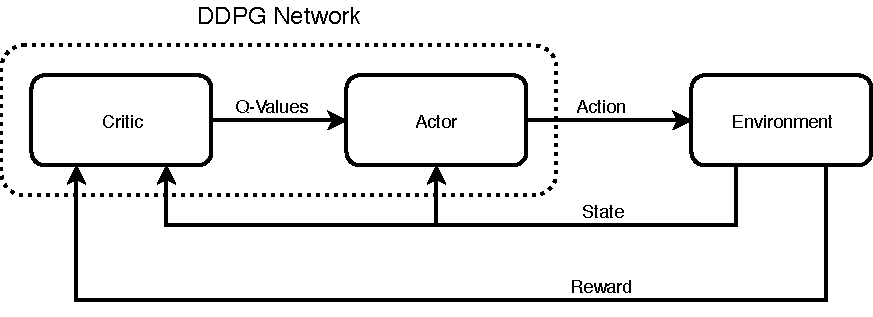
\includegraphics[width=6in, height=3.5in, keepaspectratio]{figures/actor_critic.pdf}
	\caption{Actor-Critic Architecture}\label{fig:actor_critic}
\end{figure}

The two major steps in any actor-critic method are actor improvement and critic evaluation \cite{actor_critic}. During actor improvement, the Q-values (more specifically, the gradient thereof) produced by the critic are used to train the actor network to better follow the policy. During critic evaluation, the critic, which is really just a Q-approximator as implemented in DQN, is improved using the Bellman equation. Conceptually, the actor and critic are much like a basketball player and coach. The coach learns the game and comes up with a strategy while the player focuses on executing the plan as best as possible.

Additionally, Lillicrap et al.\ adapted batch normalization from Ioffe's work to allow ANN hyper-parameter generalization for environments with features of varying magnitude \cite{2015arXiv150203167I}; each feature in a minibatch is normalized to unit mean and variance. In other words, the DDPG algorithm can use the same set of hyper-parameters, e.g. learning rates, discount factor, update parameter $\tau$, etc., for widely different environments. In their implementation, batch normalization was applied to network inputs, all layers of the policy network, and all layers of the Q network before the action input (detailed later).

To ensure adequate exploration, Lillicrap et al.\ added Ornstein-Uhlenbeck process noise to the policy output $\mu(s_t | \theta^\mu_t)$ to create the exploration policy $\mu'(s_t)$ as shown in Equation \ref{eq:exploration_policy} \cite{lillicrap_2016}. The Ornstein-Uhlenbeck process satisfies the condition shown in Equation \ref{eq:ornstein-uhlenbeck} where $x_t$ is the process position at time $t$, $\theta$ and $\sigma$ are parameters, and $W_t$ is the Weiner process \cite{uhlenbeck_ornstein}. The process produces random, time-correlated values that drift toward a long-term mean, in this case 0. The Ornstein-Uhlenbeck action noise class shown in Listing \ref{list:ornstein-uhlenbeck} is provided by OpenAI under the MIT License \cite{ddpg_noise}.
\begin{equation}
\label{eq:exploration_policy}
\mu'(s_t) = \mu(s_t | \theta^\mu_t) + \mathcal{N}
\end{equation}
\begin{equation}
\label{eq:ornstein-uhlenbeck}
dx_t = \theta(\mu-x_t) dt + \sigma dW_t, \theta>0, \sigma>0
\end{equation}

Lillicrap et al.\ used DDPG to solve over 25 different simulated physics environments such as cart pole swing-up and driving using the same network architecture and hyper-parameters, demonstrating the generalizability of the technique. For details of the environments, see OpenAI Gym \cite{openaigym}. Although the approach required about 2.5 million steps of experience to solve most problems, this represents 20 times less than DQN while still providing better performance in most cases.

To reiterate, the important advantage of the DDPG technique is its ability to handle both continuous action and state spaces of varying magnitude, critical to many real-life control problems. Specific algorithm details are covered in the Implementation section.

\begin{python}[caption={Ornstein-Uhlenbeck Action Noise \cite{ddpg_noise}},label={list:ornstein-uhlenbeck}]
class OrnsteinUhlenbeckActionNoise:
    def __init__(self, mu, sigma=0.3, theta=.15, dt=0.05, x0=None):
        self.theta = theta
        self.mu = mu
        self.sigma = sigma
        self.dt = dt
        self.x0 = x0
        self.reset()

    def __call__(self):
        x = self.x_prev + self.theta * (self.mu - self.x_prev) * self.dt + \
                self.sigma * np.sqrt(self.dt) * np.random.normal(size=self.mu.shape)
        self.x_prev = x
        return x

    def reset(self):
        self.x_prev = self.x0 if self.x0 is not None else np.zeros_like(self.mu)

    def __repr__(self):
        return 'OrnsteinUhlenbeckActionNoise(mu={}, sigma={})'.format(self.mu, self.sigma)
\end{python}

\section{Implementation}
All code is implemented in Python 3.6 and uses modules from TensorFlow \cite{tensorflow} (ANN implementation), OpenAI Gym (Ornstein-Uhlenbeck action noise) \cite{openaigym}, and Pyglet (environment rendering). An implementation of Lillicrap's DDPG algorithm from Patrick Emami's reinforcement learning primer formed the initial code base to which modifications and new developments were added \cite{emami_2016}.


\subsection{Coordinate Definitions}
The Roborodentia field is 2438.4 mm long in the $x$ direction and 1219.2 mm wide in $y$ as shown in Figure \ref{fig:field_defs} \cite{roborodentia}. Viewed from above, the coordinate (0 mm, 0 mm) is the bottom-left corner while (2438.4 mm, 1219.2 mm) is the top-right. Units of position ($x$ and $y$), orientation, linear velocity, and rotational velocity are mm, mm/s, radians, and radians/s, respectively.

The robot position and orientation, ($x$, $y$, $\theta$), is represented as a vector in the field plane where the vector's tail is positioned at the robot center and tip at the robot's front. Note that the vector orientation deviates from standard notation. At 0 radians, the vector points in the $+y$ direction, and at $+\pi/2$ radians, it points towards $-x$. 

The $x$ and $y$ velocity of the robot refer to motion parallel to the field's x-axis and y-axis while the rotational velocity refers to the robot's rotation about its center. They are defined as $\dot{x}$, $\dot{y}$, and $\dot{\theta}$. 

Three control inputs $u_x$, $u_y$, and $u_\theta$ correspond to the force applied to the robot and range between -2 to +2. For absolute clarity, positive $u_x$ moves the robot in the direction of the positive x-axis, positive $u_y$ pushes towards the positive y-axis, and positive $u_\theta$ torques the robot in the positive $\theta$ direction. 
\begin{figure}[H]
	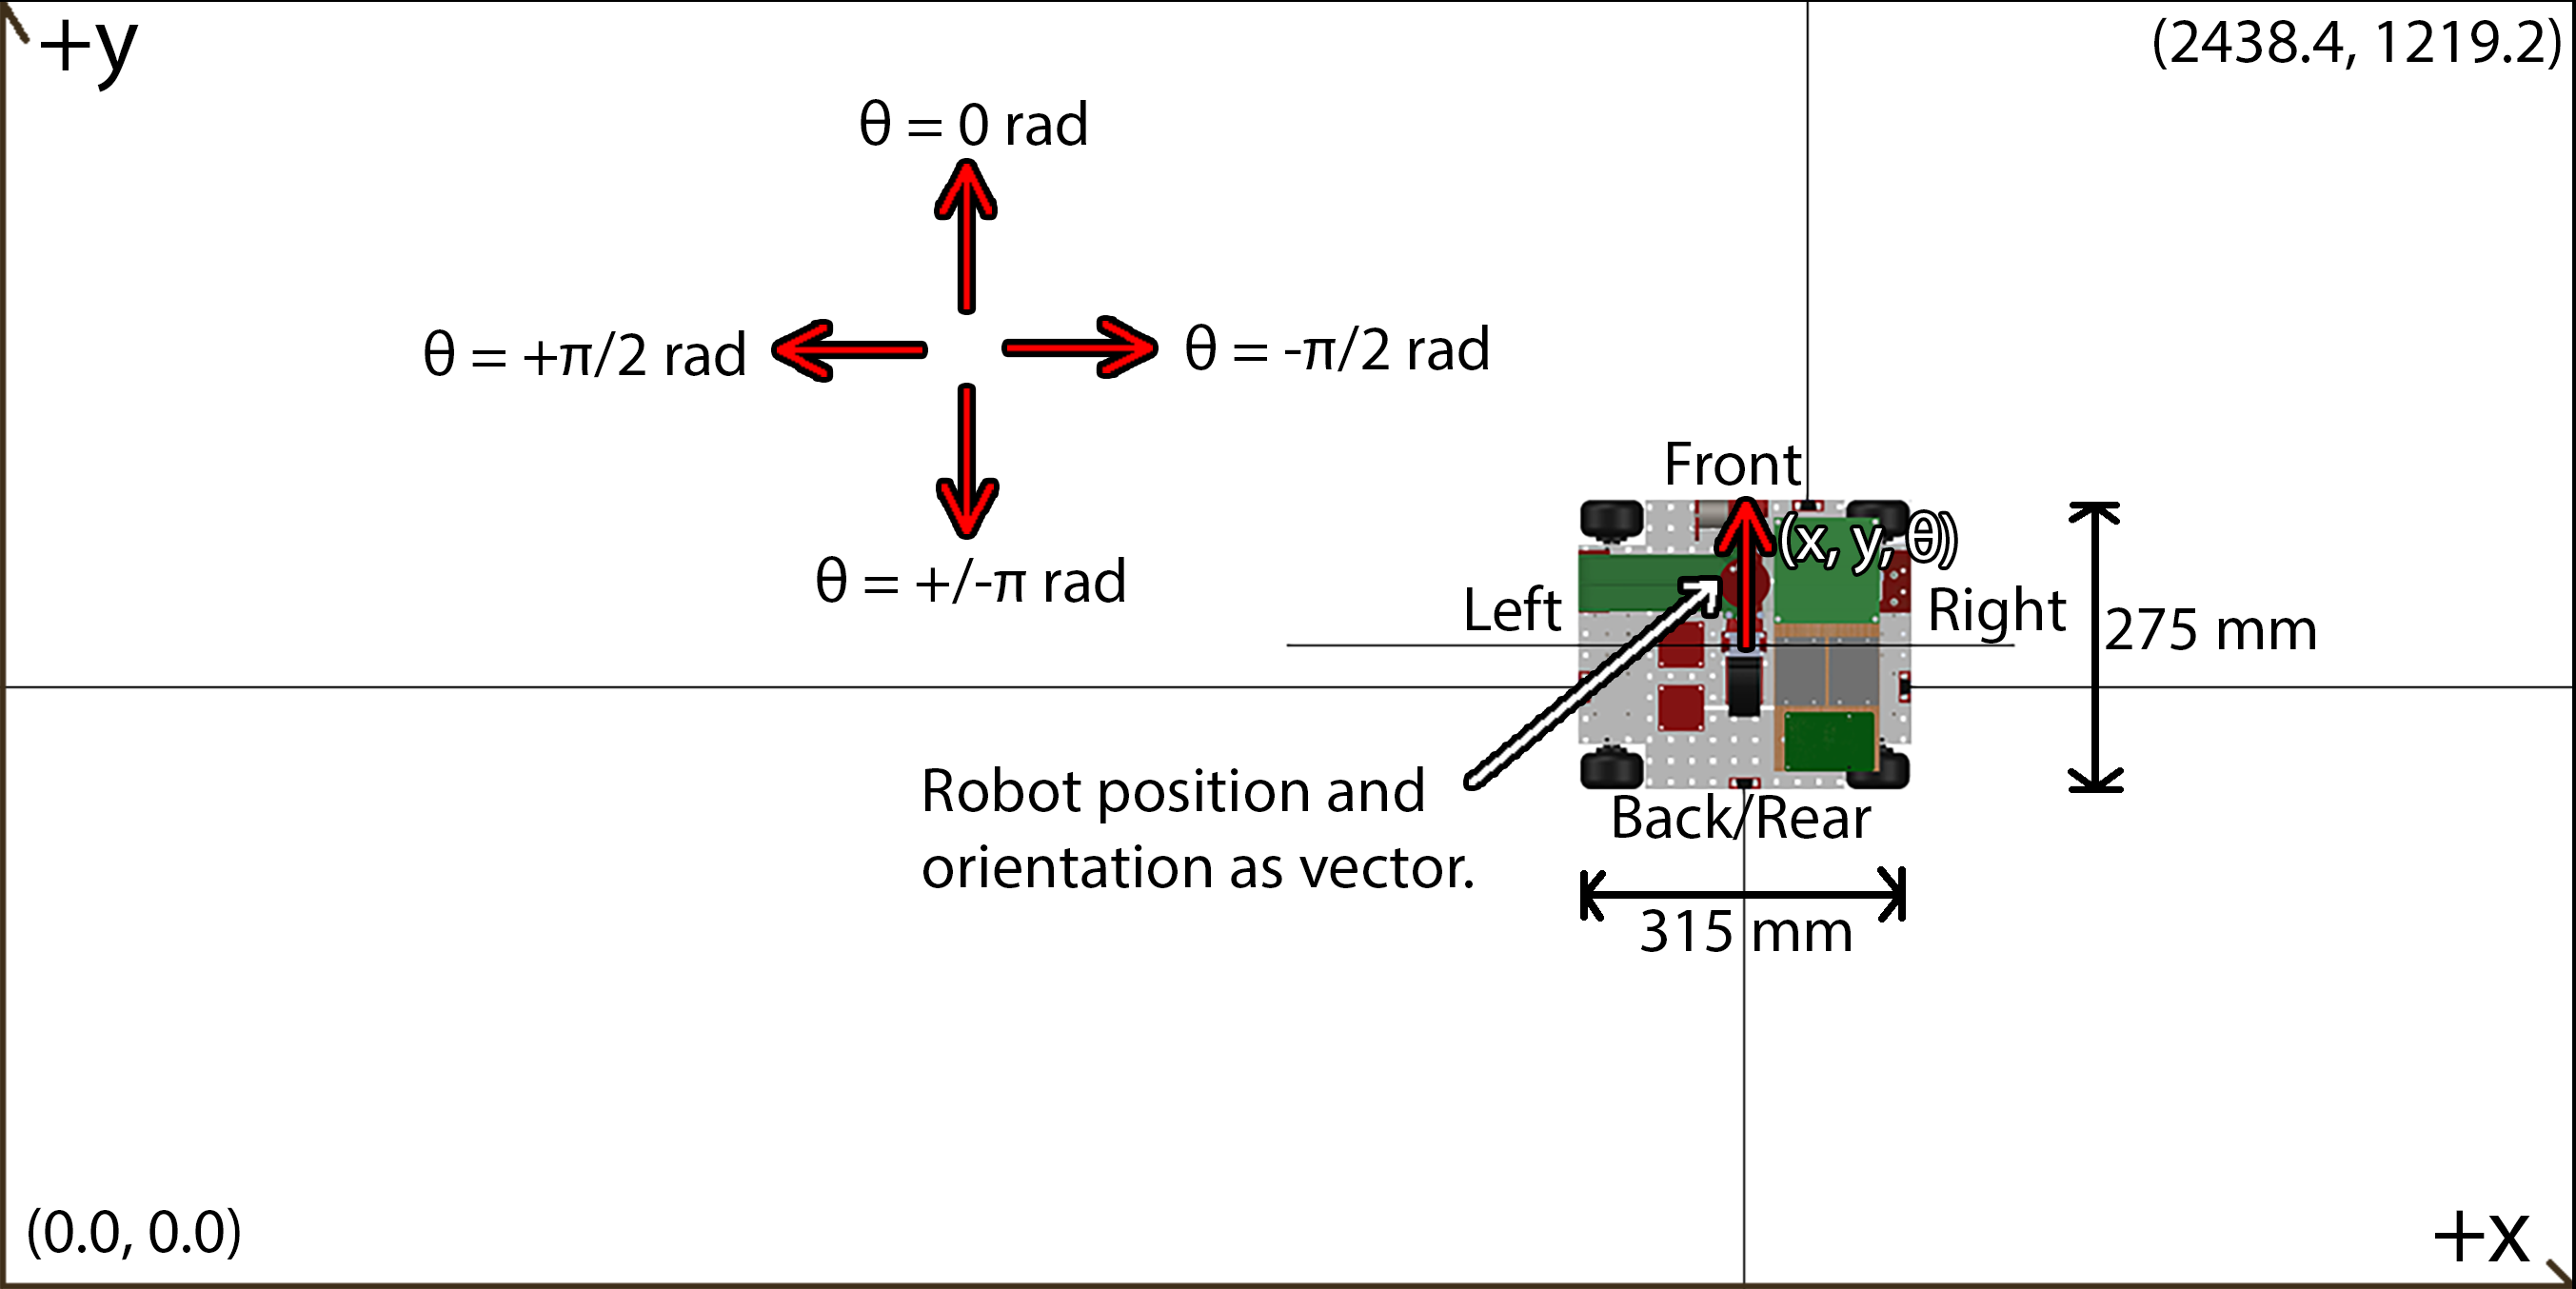
\includegraphics[width=6in, height=3.85in, keepaspectratio]{figures/field_defs.png}
	\caption{Roborodentia Field Definitions} \label{fig:field_defs}
\end{figure}

\subsection{Robot Simulation}
Since training the network using the real-life robot is difficult and time-consuming, episodes take place in a simulation of the robot and competition field. While an ideal simulation would model many kinematics and dynamics of the robot, robust system modeling is beyond the scope of the thesis. Instead, a rudimentary model serves to demonstrate the efficacy of the DDPG algorithm. 

The simulation accounts for maximum wheel velocity and acceleration and calculates robot movement as a function of the four wheel velocities using the mecanum wheel equations \cite{li_2018}\cite{rahman_2014}. It also handles collision with the environment walls. The simulation does not model unequal loading and friction between wheels, the momentum of the robot as a whole, or small differences between the motors and wheels.

\subsection{Reward Assignment}
The reward assignment must reflect the actor's goal: to move the robot to a desired position and orientation in the field. The resulting policy after training depends greatly on careful selection of which actions and/or states receive better or worse rewards. The rewards as implemented, shown in Equations \ref{eq:reward_x} to \ref{eq:reward_uth}, consist of three categories: distance from the set point, velocity, and action value. Note that the $\text{norm}(\cdot)$ function normalizes the angle to between $-\pi$ and $+\pi$. Each of the nine reward equations produces a maximum reward of 0 and includes squared terms to introduce quadratic reward scaling.

The coefficients for $r_\theta$, $r_{\dot{\theta}}$, and $r_{u_\theta}$ come from OpenAI Gym's pendulum environment \cite{openai_pendulum}. The other coefficients scale the reward magnitudes within each category close to each other. For example, the minimum $r_{y} = -0.00001 (1200 - 0)^2 = -14.4$ while the minimum $r_{\theta} = -1.0 (\pi)^2 = -9.9$. Finally, the coefficients were adjusted through trial-and-error: the algorithm was run multiple times with slightly varied coefficients until the author felt the policy was ``good enough''. Future work includes a more systematic way to determine these coefficients.
\begin{align}
r_x &= -0.00001 (x-x_{desired})^2 \label{eq:reward_x}\\
r_y &= -0.00001 (y-y_{desired})^2 \\
r_\theta &= -1.0 (norm(\theta)-norm(\theta_{desired}))^2 \\
r_{\dot{x}} &= -0.0000005 \dot{x}^2 \\
r_{\dot{y}} &= -0.0000005 \dot{y}^2 \\
r_{\dot{\theta}} &= -0.1 \dot{\theta}^2 \\
r_{u_x} &= -0.001u_x^2 \\
r_{u_y} &= -0.001u_y^2 \\
r_{u_\theta} &= -0.001u_\theta^2 \label{eq:reward_uth}
\end{align}

\subsection{Artificial Neural Networks}
\subsubsection{Critic Network}
Listing \ref{list:critic_net} implements the critic network class. The function \\
\mbox{\pythoninline{create_critic_network()}} at line 55 instantiates the TensorFlow network graph. The critic consists of a \mbox{\pythoninline{s_dim}-node} state input layer, another \mbox{\pythoninline{a_dim}-node} action input layer, two fully connected hidden layers, and a 1-node output layer, illustrated in Figure \ref{fig:critic_net}. The state input layer enters into the first hidden layer while the action input layer connects to the second hidden layer. The first hidden layer uses a fully connected network layer of weights with biases, a batch normalization layer described previously in Section \ref{sec:ddpg}, and the Rectified Linear Unit (ReLU) activation function $ReLU(x) = max(0,x)$. Deep neural networks widely use the ReLU function for speeding up large computations both in forward and backward passes of the network \cite{2017arXiv171005941R}. The derivative of the ReLU function is simply 1 for positive inputs and 0 otherwise, greatly simplifying the back propagation algorithm. The second hidden layer consists of 600 nodes, half of which connect to the first hidden layer output and half that connect to the action input layer. Finally, the output layer is a single node with no activation function to obtain linear output.

The \pythoninline{action_gradients()} function returns a list of the gradients of the output with respect to each action, used by the actor network to update its weights. Finally, the \pythoninline{train()} function optimizes network weights and biases to minimize the loss function using the Adam optimizer \cite{adam_opt}. The loss is defined as the mean square value of the difference between the mini-batch of critic outputs and the mini-batch of predicted Q-value from the target network equivalent to Equation \ref{eq:dqn_loss_func}. The Adam method, developed by Kingma and Ba, stands for ``adaptive moment estimation'' and possesses many of the benefits afforded by the AdaGrad and RMSProp algorithms including compatibility with sparse gradients, parameter update magnitudes invariant to gradient rescaling, step size annealing, and bounded step size \cite{duchi_2011}\cite{adam_opt}\cite{tieleman_2012}.
\begin{figure}[H]   % [h] means here
	\centering 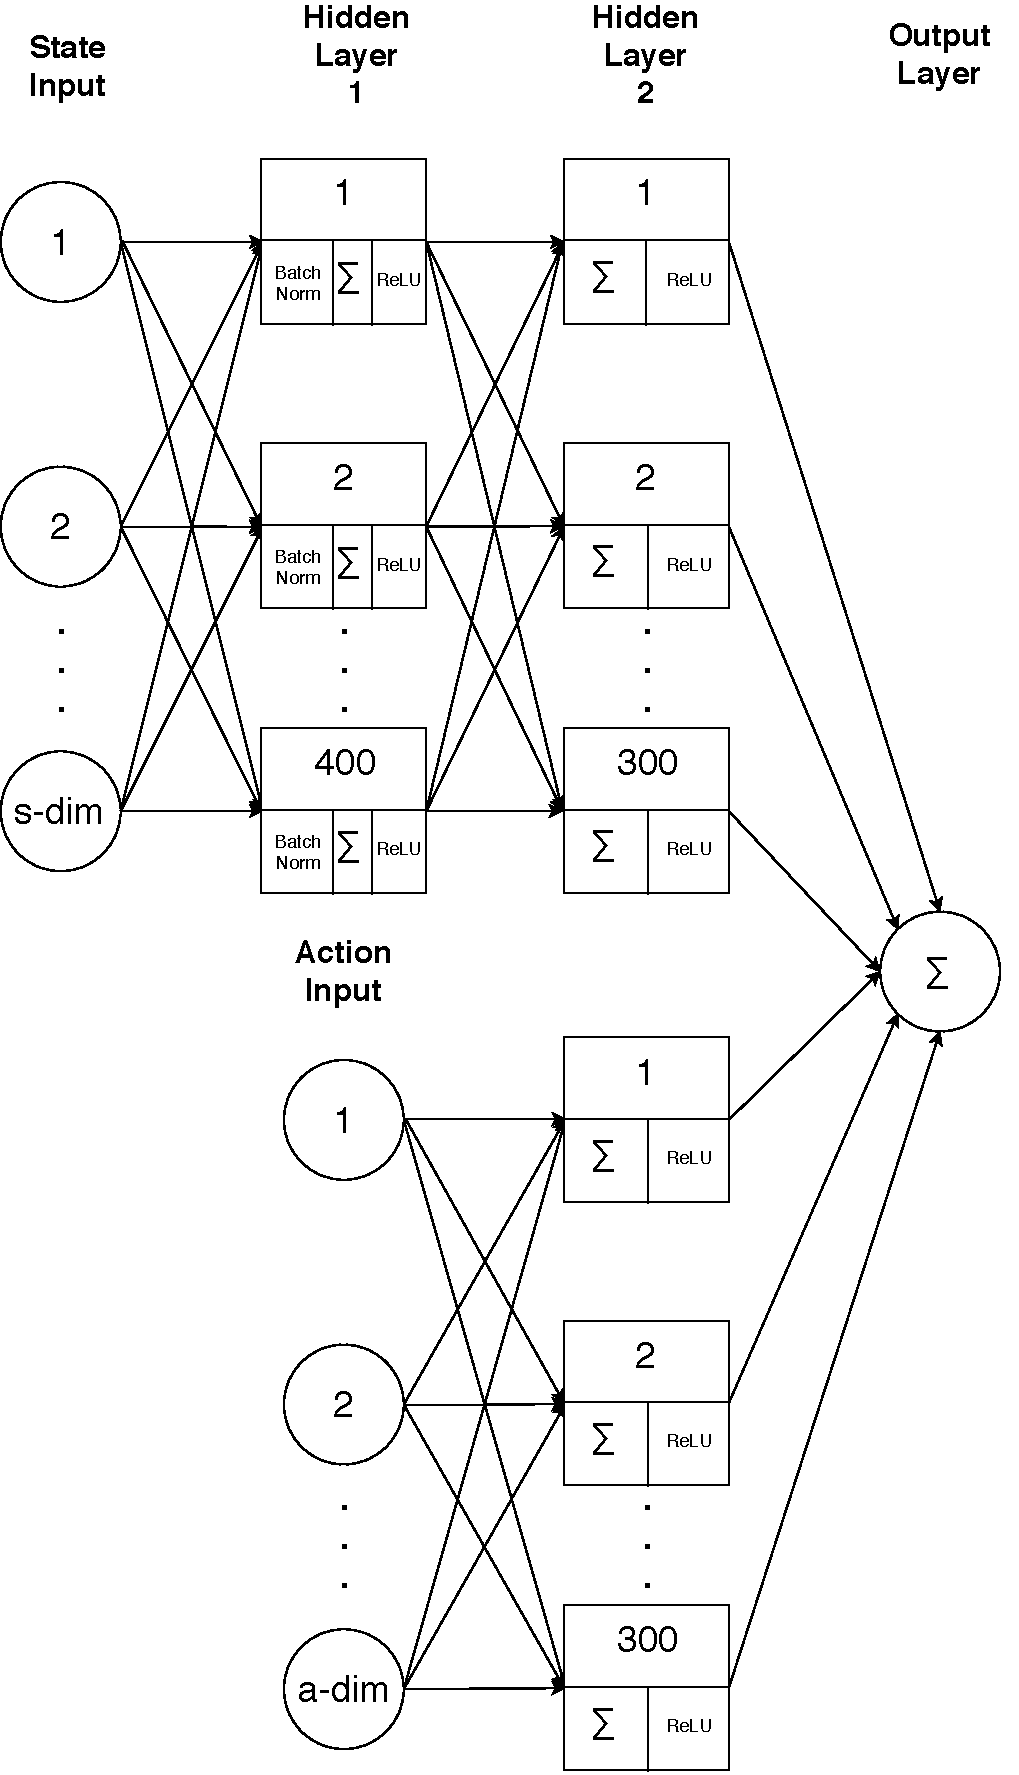
\includegraphics[width=6in, height=8.5in, keepaspectratio]{figures/critic_net.pdf}
	\caption{Critic ANN Structure}\label{fig:critic_net}
\end{figure}

\begin{python}[caption={Critic Network Class},label={list:critic_net}]
CRITIC_L1_NODES = 400
CRITIC_L2_NODES = 300

class CriticNetwork(object):
    """
    Input to the network is the state and action, output is Q(s,a).
    The action must be obtained from the output of the Actor network.

    """

    def __init__(self, sess, state_dim, action_dim, learning_rate, tau, gamma, num_actor_vars):
        self.sess = sess
        self.s_dim = state_dim
        self.a_dim = action_dim
        self.learning_rate = learning_rate
        self.tau = tau
        self.gamma = gamma

        # Create the critic network
        self.inputs, self.action, self.out = self.create_critic_network()

        self.network_params = tf.trainable_variables()[num_actor_vars:]

        # Target Network
        self.target_inputs, self.target_action, self.target_out = self.create_critic_network()

        self.target_network_params = tf.trainable_variables()[(len(self.network_params) + num_actor_vars):]

        # Op for periodically updating target network with online network
        # weights with regularization
        self.update_target_network_params = [self.target_network_params[i].assign( \
            tf.multiply(self.network_params[i], self.tau) + \
            tf.multiply(self.target_network_params[i], 1. - self.tau)) \
                for i in range(len(self.target_network_params))]

        # Network target (y_i)
        self.predicted_q_value = tf.placeholder(tf.float32, [None, 1])

        # Define loss and optimization Op
        self.loss = tflearn.mean_square(self.predicted_q_value, self.out)
        self.optimize = tf.train.AdamOptimizer(
            self.learning_rate).minimize(self.loss)

        # Get the gradient of the net w.r.t. the action.
        # For each action in the mini-batch (i.e., for each x in xs),
        # this will sum up the gradients of each critic output in the mini-batch
        # w.r.t. that action. Each output is independent of all
        # actions except for one.
        self.action_grads = tf.gradients(self.out, self.action)

        self.num_trainable_vars = len(
            self.network_params) + len(self.target_network_params)


    def create_critic_network(self):
        inputs = tflearn.input_data(shape=[None, self.s_dim], name='CriticInputs')
        action = tflearn.input_data(shape=[None, self.a_dim], name='CriticAction')
        net = tflearn.fully_connected(inputs, CRITIC_L1_NODES, name='CriticInputsNet')
        net = tflearn.layers.normalization.batch_normalization(net)
        net = tflearn.activations.relu(net)

        # Add the action tensor in the 2nd hidden layer
        # Use two temp layers to get the corresponding weights and biases
        t1 = tflearn.fully_connected(net, CRITIC_L2_NODES, name='CriticNetT1')
        t2 = tflearn.fully_connected(action, CRITIC_L2_NODES, name='CriticActionT2')

        net = tflearn.activation(
            tf.matmul(net, t1.W) + tf.matmul(action, t2.W) + t2.b, activation='relu')

        # linear layer connected to 1 output representing Q(s,a)
        # Weights are init to Uniform[-3e-3, 3e-3]
        w_init = tflearn.initializations.uniform(minval=-0.003, maxval=0.003)
        out = tflearn.fully_connected(net,1, weights_init=w_init,name='CriticNetOut')
        return inputs, action, out

    def train(self, inputs, action, predicted_q_value):
        return self.sess.run([self.out, self.optimize], feed_dict={
            self.inputs: inputs,
            self.action: action,
            self.predicted_q_value: predicted_q_value
        })

    def predict(self, inputs, action):
        return self.sess.run(self.out, feed_dict={
            self.inputs: inputs,
            self.action: action
        })

    def predict_target(self, inputs, action):
        return self.sess.run(self.target_out, feed_dict={
            self.target_inputs: inputs,
            self.target_action: action
        })

    def action_gradients(self, inputs, actions):
        return self.sess.run(self.action_grads, feed_dict={
            self.inputs: inputs,
            self.action: actions
        })

    def update_target_network(self):
        self.sess.run(self.update_target_network_params)
\end{python}

\subsubsection{Actor Network}
Listing \ref{list:actor_net} implements the actor ANN. The function \pythoninline{create_actor_network()} at line 56 defines the TensorFlow graph of the network. The actor uses an \pythoninline{s_dim}-node input layer, two fully connected hidden layers, and a  \pythoninline{a_dim}-node output layer, illustrated in Figure \ref{fig:actor_net}. The two hidden layers consist of a fully connected network layer of weights with biases, a batch normalization layer described previously, and the ReLU activation function. The two hidden layers use 400 and 300 nodes, respectively, matching Lillicrap's implementation \cite{lillicrap_2016}. Finally, the output layer is a fully connected network, $\text{tanh}(\cdot)$ activation function to limit the output to $[-1,+1]$, and a multiplier to scale the output to $[-$\pythoninline{action_bound}$,+$\pythoninline{action_bound}$]$.

The \pythoninline{train()} function implements the key idea of the policy gradient method. The gradient of the output with respect to the network weights and biases are calculated and weighted the by the action gradients obtained from the critic. The weighting step effectively makes ``good'' actions more likely and ``bad'' actions less likely. The gradients are normalized by the batch size and then applied to the network weights and biased according to the Adam optimization method. 
\begin{figure}[H]   % [h] means here
	\centering 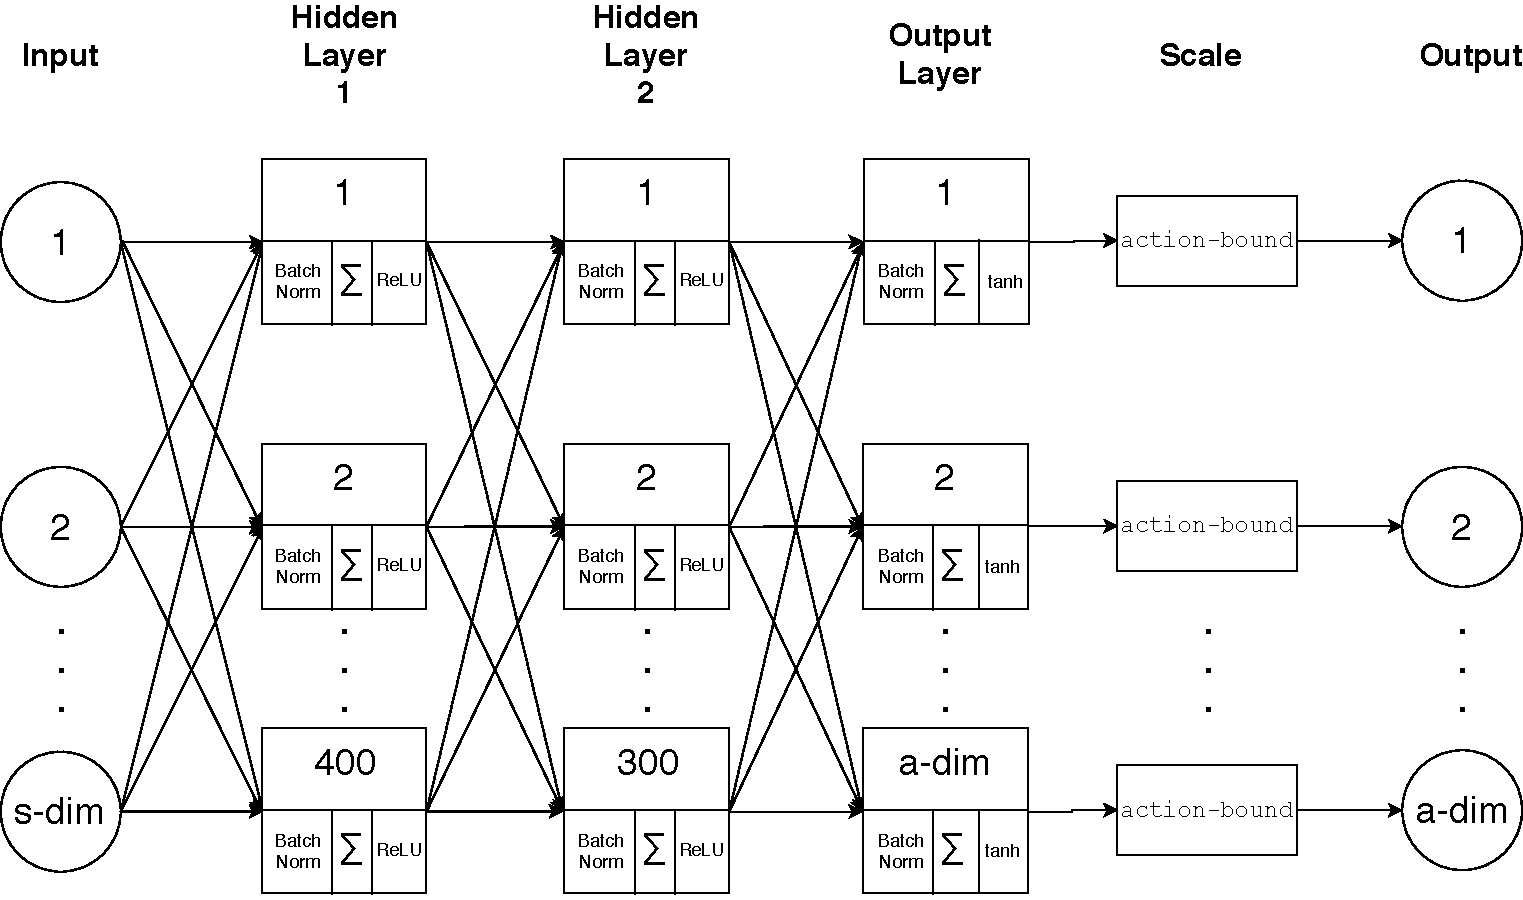
\includegraphics[width=6in, height=3.85in, keepaspectratio]{figures/actor_net.pdf}
	\caption{Actor ANN Structure}\label{fig:actor_net}
\end{figure}
\newpage
\begin{python}[caption={Actor Network Class},label={list:actor_net}]
ACTOR_L1_NODES = 400
ACTOR_L2_NODES = 300

class ActorNetwork(object):
    """
    Input to the network is the state, output is the action
    under a deterministic policy.

    The output layer activation is a tanh to keep the action
    between -action_bound and action_bound
    """

    def __init__(self, sess, state_dim, action_dim, action_bound, learning_rate, tau, batch_size):
        self.sess = sess
        self.s_dim = state_dim
        self.a_dim = action_dim
        self.action_bound = action_bound
        self.learning_rate = learning_rate
        self.tau = tau
        self.batch_size = batch_size

        # Actor Network
        self.inputs, self.out, self.scaled_out = self.create_actor_network()

        self.network_params = tf.trainable_variables()

        # Target Network
        self.target_inputs, self.target_out, self.target_scaled_out = self.create_actor_network()

        self.target_network_params = tf.trainable_variables()[
            len(self.network_params):]

        # Op for periodically updating target network with online network
        # weights
        self.update_target_network_params = [self.target_network_params[i].assign( \
                tf.multiply(self.network_params[i], self.tau) + \
                tf.multiply(self.target_network_params[i], 1. - self.tau))
                for i in range(len(self.target_network_params))]

        # This gradient will be provided by the critic network
        self.action_gradient = tf.placeholder(tf.float32, [None, self.a_dim])

        # Combine the gradients here
        self.unnormalized_actor_gradients = tf.gradients(
            self.scaled_out, self.network_params, -self.action_gradient)
        self.actor_gradients = list(map(lambda x: tf.div(x, self.batch_size), 
            self.unnormalized_actor_gradients))

        # Optimization Op
        self.optimize = tf.train.AdamOptimizer(self.learning_rate).\
            apply_gradients(zip(self.actor_gradients, self.network_params))

        self.num_trainable_vars = len(
            self.network_params) + len(self.target_network_params)

    def create_actor_network(self):
        inputs = tflearn.input_data(shape=[None, self.s_dim], name='ActorInputs')
        net = tflearn.fully_connected(inputs, ACTOR_L1_NODES, name='ActorInputsNet')
        net = tflearn.layers.normalization.batch_normalization(net, name='ActorBatchNorm1Net')
        net = tflearn.activations.relu(net)
        net = tflearn.fully_connected(net, ACTOR_L2_NODES, name='ActorNetNet')
        net = tflearn.layers.normalization.batch_normalization(net, name='ActorBatchNorm2Net')
        net = tflearn.activations.relu(net)
        # Final layer weights are init to Uniform[-3e-3, 3e-3]
        w_init = tflearn.initializations.uniform(minval=-0.003, maxval=0.003)
        out = tflearn.fully_connected(
            net, self.a_dim, activation='tanh', weights_init=w_init, name='ActorOutNet')
        # Scale output to -action_bound to action_bound
        scaled_out = tf.multiply(out, self.action_bound)
        return inputs, out, scaled_out

    def train(self, inputs, a_gradient):
        self.sess.run(self.optimize, feed_dict={
            self.inputs: inputs,
            self.action_gradient: a_gradient
        })

    def predict(self, inputs):
        return self.sess.run(self.scaled_out, feed_dict={
            self.inputs: inputs
        })

    def predict_target(self, inputs):
        return self.sess.run(self.target_scaled_out, feed_dict={
            self.target_inputs: inputs
        })

    def update_target_network(self):
        self.sess.run(self.update_target_network_params)

    def get_num_trainable_vars(self):
        return self.num_trainable_vars
\end{python}

Both actor and critic classes create a regular and target network in the \mbox{\pythoninline{__init__()}} function. Each target network is structurally identical to its respective actor or critic network. Recall the network weights are denoted as $\theta_i$ while target network weights use $\theta^-_i$. Each class provides a function \pythoninline{update_target_network()}  that adjusts target network weights to be closer to the regular network weights by the factor $\tau=0.001$ as in Equation \ref{eq:target_update}. The \pythoninline{predict()} and \pythoninline{predict_targets()} functions return the forward pass output of the regular and target networks, respectively.
\begin{equation}
\label{eq:target_update}
\theta^-_i \gets \tau\theta_i + (1-\tau)\theta^-_i
\end{equation}

\subsection{DDPG}
Figure \ref{fig:ddpg_flow} displays the DDPG training algorithm flowchart. The network testing section is not core to DDPG but provides helpful insight into the change in system performance throughout training. The program continues training the network indefinitely until the user quits the program. The list below details algorithm steps with accompanying code snippets.
\begin{enumerate}
\item Set training parameters such as learning rates, discount factor $\gamma$, target network update parameter $\tau$, and mini-batch size. The arguments use default values unless specified in the program arguments list.
\begin{python}[caption={Training Parameter Initialization},label={list:train_param_init},xleftmargin=\dimexpr-\csname @totalleftmargin\endcsname]
parser.add_argument('--actor-lr', help='actor network learning rate', default=0.001) 
parser.add_argument('--critic-lr', help='critic network learning rate', default=0.0001) 
parser.add_argument('--gamma', help='discount factor for critic updates', default=0.99) 
parser.add_argument('--tau', help='soft target update parameter', default=0.001) 
parser.add_argument('--buffer-size', help='max size of the replay buffer', default=1000000)
parser.add_argument('--minibatch-size', help='size of minibatch for minibatch-SGD', default=64)
\end{python}
\item Initialize the actor network, critic network, Ornstein-Uhlenbeck exploration noise, and experience replay buffer. Set the random seed to a specific value for repeatability.
\begin{python}[caption={Network, Noise, and Experience Replay Buffer Initialization},label={list:net_init},xleftmargin=\dimexpr-\csname @totalleftmargin\endcsname]
print("Instantiating actor...")
actor = ActorNetwork(sess, state_dim, action_dim, action_bound,
                     float(args['actor_lr']), float(args['tau']),
                     int(args['minibatch_size']))

print("Instantiating critic...")
critic = CriticNetwork(sess, state_dim, action_dim,
                       float(args['critic_lr']), float(args['tau']),
                       float(args['gamma']),
                       actor.get_num_trainable_vars())
actor_noise = OrnsteinUhlenbeckActionNoise(mu=np.zeros(action_dim), dt=env.dt)
replay_buffer = ReplayBuffer(int(args['buffer_size']), int(args['random_seed']))
\end{python}
\item Initialize TensorFlow variables and \pythoninline{tf.train.Saver()} for saving trained models to disk.
\begin{python}[caption={Saver Initialization},label={list:saver_init},xleftmargin=\dimexpr-\csname @totalleftmargin\endcsname]
sess.run(tf.global_variables_initializer())
saver = tf.train.Saver()
\end{python}
\item Start training loop. Each run of this loop is one episode.
	\begin{enumerate}
	\item Reset the environment randomly and get the initial state. Reset the episode reward and average maximum Q, described in Section \ref{sec:xtrans_results}, for each step. These two quantities are not part of the network itself but are used to track actor performance. 
	\begin{python}[caption={Episode Reset},label={list:ep_reset},xleftmargin=\dimexpr-\csname @totalleftmargin\endcsname]
s = env.reset()

# Track the episode reward and average max q
ep_reward = 0
ep_ave_max_q = 0
	\end{python}
	\item Start step loop. Each run of this loop is one step in the episode.
		\begin{enumerate}
		\item Predict an action (i.e. forward pass through actor network) and add Ornstein-Uhlenbeck exploration noise. Execute the action and receive a reward, next state, and if the environment is terminating. Add the transition to the experience replay buffer.
		\begin{python}[caption={Actor Predict and Step},label={list:act_pred_step},xleftmargin=\dimexpr-\csname @totalleftmargin\endcsname]
# Predict action and add exploration noise
a = actor.predict(np.reshape(s, (1, actor.s_dim))) + actor_noise()
action = a[0]

# Execute action in environment to change state
s2, r, terminal, info = env.step(action)

replay_buffer.add(np.reshape(s, (actor.s_dim,)), \
        np.reshape(action, (actor.a_dim,)), r, terminal, \
        np.reshape(s2, (actor.s_dim,)))
		\end{python}
		\item If the experience replay buffer contains at least the mini-batch number of transitions, sample a mini-batch of transitions. Use the target critic network to produce a target Q and calculate $y_i$ from the mini-batch of transitions for use in the critic loss function. Update critic and actor network weights then target critic and actor weights.
		\begin{python}[caption={Network Update},label={list:net_update},xleftmargin=\dimexpr-\csname @totalleftmargin\endcsname]
# Keep adding experience to the memory until
# there are at least minibatch size samples
if replay_buffer.size() > int(args['minibatch_size']):
	s_batch, a_batch, r_batch, t_batch, s2_batch = \
	  	replay_buffer.sample_batch(int(args['minibatch_size']))
	
	# Calculate targets
	target_q = critic.predict_target(
	  	s2_batch, actor.predict_target(s2_batch))
	
	y_i = []
	for k in range(int(args['minibatch_size'])):
	  	if t_batch[k]:
	      	y_i.append(r_batch[k])
	  	else:
	      	y_i.append(r_batch[k] + critic.gamma * target_q[k])
	
	# Update the critic given the targets
	predicted_q_value, _ = critic.train( s_batch, a_batch, \
	  	np.reshape(y_i, (int(args['minibatch_size']), 1)))
	
	ep_ave_max_q += np.amax(predicted_q_value)
	
	# Update the actor policy using the sampled gradient
	a_outs = actor.predict(s_batch)
	grads = critic.action_gradients(s_batch, a_outs)
	actor.train(s_batch, grads[0])
	
	# Update target networks
	actor.update_target_network()
	critic.update_target_network()
		\end{python}	
		\end{enumerate}
	\item Update state for the next step and increment episode reward.
	\begin{python}[caption={Step Cleanup},label={list:ep_clean},xleftmargin=\dimexpr-\csname @totalleftmargin\endcsname]
# Update state for next step
s = s2

# Increment episode reward
ep_reward += r
	\end{python}
	\item If the environment is terminated, break out of the episode. Otherwise, loop back.
	\begin{python}[caption={Episode Termination},label={list:ep_term},xleftmargin=\dimexpr-\csname @totalleftmargin\endcsname]
# End of episode
if terminal:
  	break
	\end{python}
	\item Print episode information to track progress.
	\begin{python}[caption={Print Episode Results},label={list:print_ep},xleftmargin=\dimexpr-\csname @totalleftmargin\endcsname]
print('Ep: %d | Reward: %d | Qmax: %0.4f' % \
	(i, int(ep_reward), ep_ave_max_q / float(ep_len)))
	\end{python}
	\item Periodically test the network performance (detailed in the subsection Actor Testing), record test results, save network weights to file, and produce contour plots of actor and critic outputs.
	\begin{python}[caption={Network Evaluation},label={list:net_eval},xleftmargin=\dimexpr-\csname @totalleftmargin\endcsname]
# Test the network's performance
if (i % test_period == 0):
    # Test the network and get the total reward
    print("Testing network in %d cases..." % (num_test_cases))
    test_reward, episodes = testNetworkPerformance(env, args, actor, num_test_cases)
    plotEpisodes(env.net_index, episodes, env.dt, i+1)

    # Save network session
    filepath = "./results/%s/%s_%d_%d/model.ckpt" % (sess_dir, args['env'], i+1,int(test_reward))
    save_path = saver.save(sess, filepath)

    # Contour plots of ANN output
    if (args['env'] != 'all'):
        plotANN(env.net_index, actor, i+1, 0)
        plotANN(env.net_index, critic, i+1, 1)
	\end{python}	
	\end{enumerate}
\end{enumerate}
\begin{figure}[H]   % [h] means here
	\centering 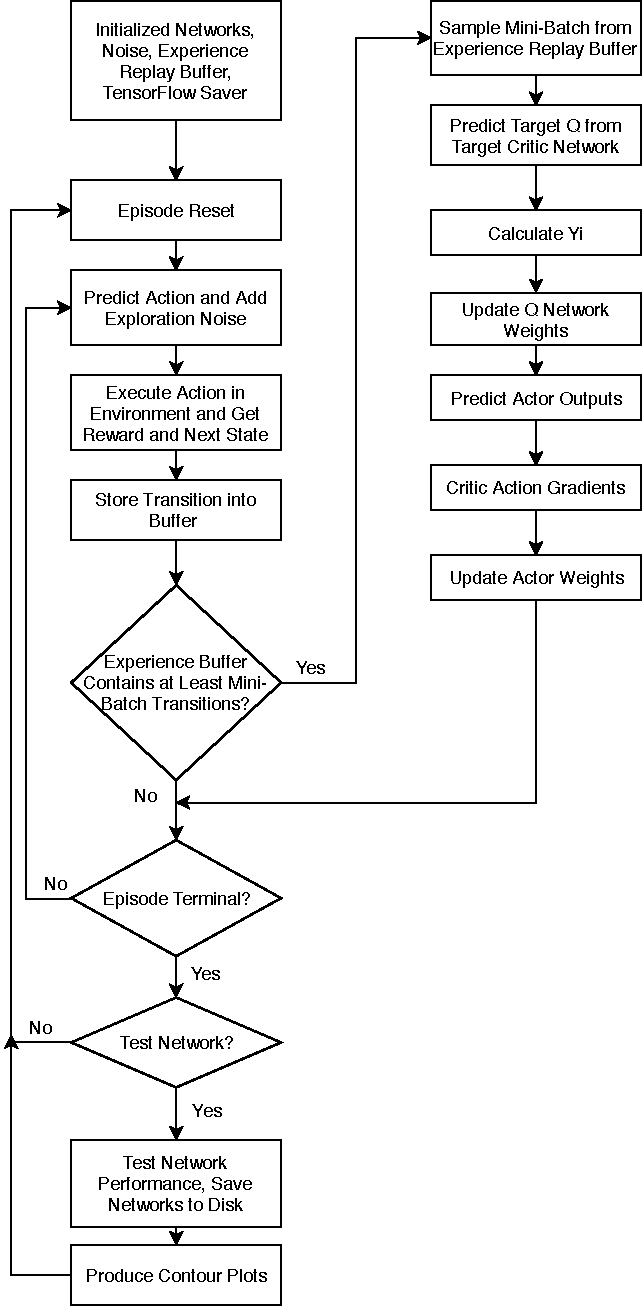
\includegraphics[width=6in, height=8.5in, keepaspectratio]{figures/ddpg_flow.pdf}
	\caption{DDPG Flowchart}\label{fig:ddpg_flow}
\end{figure}

\subsection{Two Approaches}
Since the robot's mecanum wheels permit omni-directional movement, position and orientation control can be broken down into three separate DDPG actors, referred to as the ``x translation'', ``y translation'', and ``rotation'' or ``angle'' networks. Each actor receives two state inputs: position ($x$, $y$, or $\theta$) and velocity ($\dot{x}$, $\dot{y}$, or $\dot{\theta}$) and outputs one of three orthogonal controls ($u_x$, $u_y$, and $u_\theta$). This will be referred to as the ``three actors'' approach. Each of the three networks trains in isolation from the other two; for example, when training the x translation network, $u_y$ and $u_\theta$ are fixed at 0.

After the networks generate the control signals, some post-processing is required to simultaneously apply the effects of each control. They are converted to four individual motor voltages ($v_0$, $v_1$, $v_2$, and $v_3$) by calculating the translation vector magnitude $V_d = \sqrt{u_x^2 + u_y^2}/2$ and angle $\theta_d = \text{atan2}(u_y / u_x)$ then using Equations \ref{eq:mecanum_v0} through \ref{eq:mecanum_v3} \cite{li_2018}\cite{rahman_2014}. The desired voltages are then communicated to the microcontroller which generates the appropriate signals.
\begin{align}
v_0 &= V_d \text{sin}(\theta_d + \pi/4) - u_\theta  \label{eq:mecanum_v0}\\
v_1 &= V_d \text{cos}(\theta_d + \pi/4) + u_\theta  \label{eq:mecanum_v1}\\
v_2 &= V_d \text{sin}(\theta_d + \pi/4) + u_\theta  \label{eq:mecanum_v2}\\
v_3 &= V_d \text{cos}(\theta_d + \pi/4) - u_\theta  \label{eq:mecanum_v3}
\end{align}

In the alternative ``single actor'' approach, a single actor receives $x$, $y$, $\theta$, $\dot{x}$, $\dot{y}$, and $\dot{\theta}$ then produces the three control components $u_x$, $u_y$, and $u_\theta$. 

The three actor approach provides a few significant benefits over the single actor. First, it allows for partial system retraining. For example, if the y translation network does not meet the design specification, it can be retrained independently whereas the single actor would require complete retraining. Additionally, separate actors simplify troubleshooting and reward assignment tuning by isolating effects and reducing problem complexity as well as improve training convergence speed. On the other hand, the approach does not account for possible effects of simultaneously-applied control components as with the single actor case. It also suffers from reduced speed due to processing three networks at each step versus just one. 

A hybrid approach would start with the three actors approach, to tune and refine the reward assignments and hyper-parameters, and finish with the single actor to reap the processing speed advantage as shown in Figure \ref{fig:hybrid_approach_flow}.
\begin{figure}[H]
	\centering
	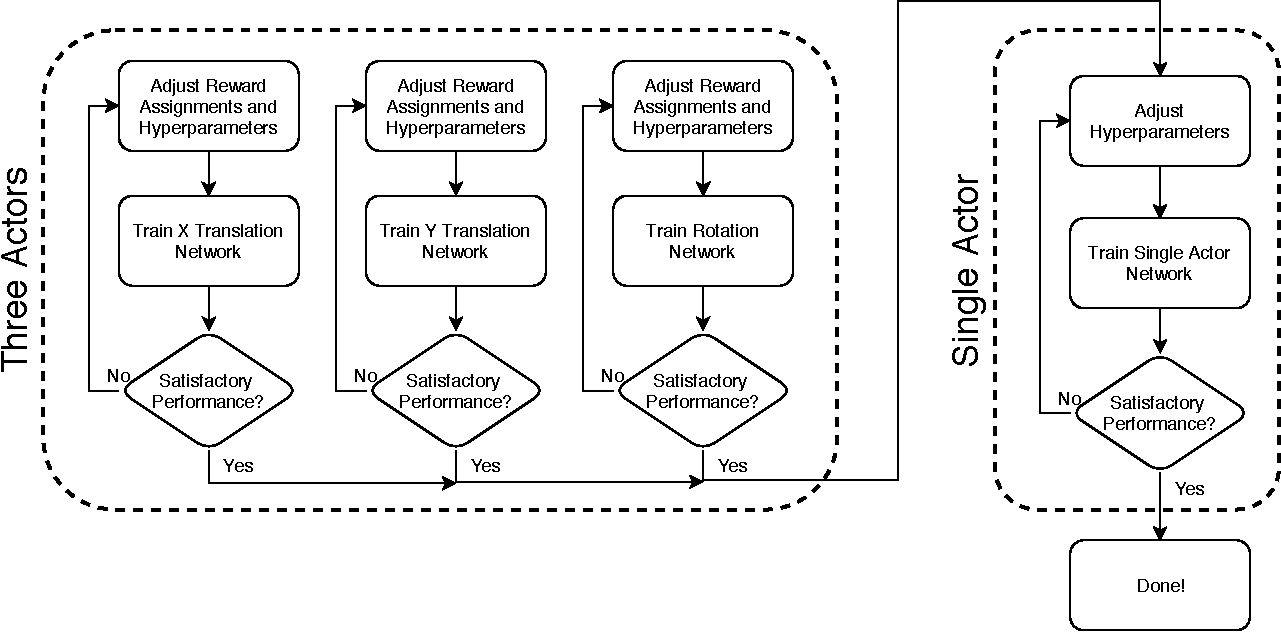
\includegraphics[width=6in, height=3.85in, keepaspectratio]{figures/hybrid_approach_flow.pdf}
	\caption{Hybrid Approach Flow} \label{fig:hybrid_approach_flow}
\end{figure}

\subsection{Training}
Each episode lasts 10 seconds with 0.05 second steps for a total of 200 steps per episode. The learning rates, discount factor, target network update parameter $\tau$, and mini-batch size for the three actors approach come from the original DDPG publication. The learning rates and $\tau$ for the single actor variant are 10 times smaller to improve stability. Table \ref{tab:training_params} summarizes the training parameters.
\begin{table}[h]
	\caption{Training Parameters}  \label{tab:training_params}
	\centering
	\begin{tabular}{l|c|c}
		\toprule
		Parameter & Three Actors & Single Actor \\ 
		\midrule
		Episode Length (s) & 10 & 10 \\
		Episode Step (s) & 0.05 & 0.05 \\
		Actor Learning Rate $\alpha_{actor}$ & $10^{-4}$ & $10^{-5}$ \\
		Critic Learning Rate $\alpha_{critic}$  & $10^{-3}$ & $10^{-4}$ \\
		Discount Factor $\gamma$ & 0.99 & 0.99 \\
		Target Network Update Parameter $\tau$ & $10^{-3}$ & $10^{-4}$ \\
		Mini-Batch Size & 64 & 128 \\
		\bottomrule
	\end{tabular} 
\end{table}

Training took place on a desktop computer with an Intel i5-4670K CPU and Nvidia GeForce GTX 980 Ti GPU running Microsoft Windows 10 Pro \cite{intel}\cite{980ti}\cite{windows}. The computer processed 21,200 episodes of single actor training in about 23 hours and 51 minutes, achieving an average rate of 1 episode every 4.08 seconds.

\subsection{Testing}
The training loop periodically tests the actor to evaluate performance with the \pythoninline{testNetworkPerformance()} function shown in Listing \ref{list:actor_testing}. The actor steps through a series of predefined test cases. For example, the robot orientation $\theta$ ranges from $-\pi$ to $+\pi$. If using 11 test cases, the robot would begin at $\theta=[-\pi, -0.8\pi, -0.6\pi,\allowbreak -0.4\pi,\allowbreak -0.2\pi,\allowbreak 0, +0.2\pi, +0.4\pi, +0.6\pi, +0.8\pi, \pi]$ to evaluate behavior at various states. Additionally, the action does not receive Ornstein-Uhlenbeck exploration noise during testing so the actor only takes greedy actions. The function returns the average reward per episode as the measure of actor performance. The testing procedure as implemented uses 41 test cases.
\begin{python}[caption={Actor Testing Function},label={list:actor_testing}]
# Tests the actor network against a number of test cases
def testNetworkPerformance(env, args, actor, num_test_cases = 10, render = False):
    test_total_reward = 0.0
    episodes = []

    # Test the network against random scenarios
    env.setWallCollision(True)
    for m in range(num_test_cases + 1):
        transitions = []
        s = env.reset(False, True, m, num_test_cases)
        ep_reward = 0.0
        for n in range(int(args['max_episode_len'])):
            if (args['render_env'] and render == True):
                env.render()

            # Choose action based on inputs
            a = actor.predict(np.reshape(s, (1, actor.s_dim)))
            action = a[0]

            # Execute action and get new state, reward
            s, r, terminal, info = env.step(action)
            ep_reward += r

            transition = (action, s, r)
            transitions.append(transition)
            if terminal:
                break
        episodes.append(transitions)
        test_total_reward += ep_reward

    env.setWallCollision(False)

    # Return the average test reward
    return (test_total_reward / (m+1), episodes)

\end{python}
%\begin{python}[caption={Caption},label={list:label}]
%
%\end{python}

\section{Results}
\subsubsection{X Translation Network} \label{sec:xtrans_results}
The $x$ translation network takes in the robot's $x$ error, the difference between the desired and actual $x$ positions, and velocity $\dot{x}$ and outputs control $u_x$. The reward is calculated as shown in Equation \ref{eq:x_reward}. The actor receives a higher reward for keeping the robot near the desired $x$ set point, minimizing the $x$ velocity, and minimizing the effort (i.e. low $u_x$ values). Since reaching the set point quickly is desirable, it may seem odd to minimize velocity. However, the velocity reward magnitude is significantly smaller than that of position, so the actor prioritizes getting to the set point quickly and later focuses on reducing speed.
\begin{equation}
r = -0.00001(x-x_{desired})^2-0.0000005\dot{x}^2-0.001u_x^2
\label{eq:x_reward}
\end{equation}

As described above in the Testing section, the networks are periodically tested to observe their change in performance with more training. Figures \ref{fig:x_r} and \ref{fig:x_rzoom} show the average testing episode reward produced by the \mbox{\pythoninline{testNetworkPerformance()}} function versus the number of episodes trained. Figure \ref{fig:x_q} shows the average max Q versus number of episodes trained. The average max Q is calculated as the average maximum Q within each mini-batch of predicted Q's. Since the algorithm is model-free and the actor starts with zero knowledge of the environment, the initial test rewards remain near -2000. However, the actor quickly learns and achieves a -58 test reward after 161 episodes. After 181 episodes, the test reward begins to decrease, indicating the possibility of over-training. Interestingly, the critic produces invalid Q estimates visible in Figure \ref{fig:x_q}; the maximum reward for any step, and therefore Q, is 0. However, this does not impact the actor's ability to determine desirable actions.
\begin{figure}[H]
	\centering
	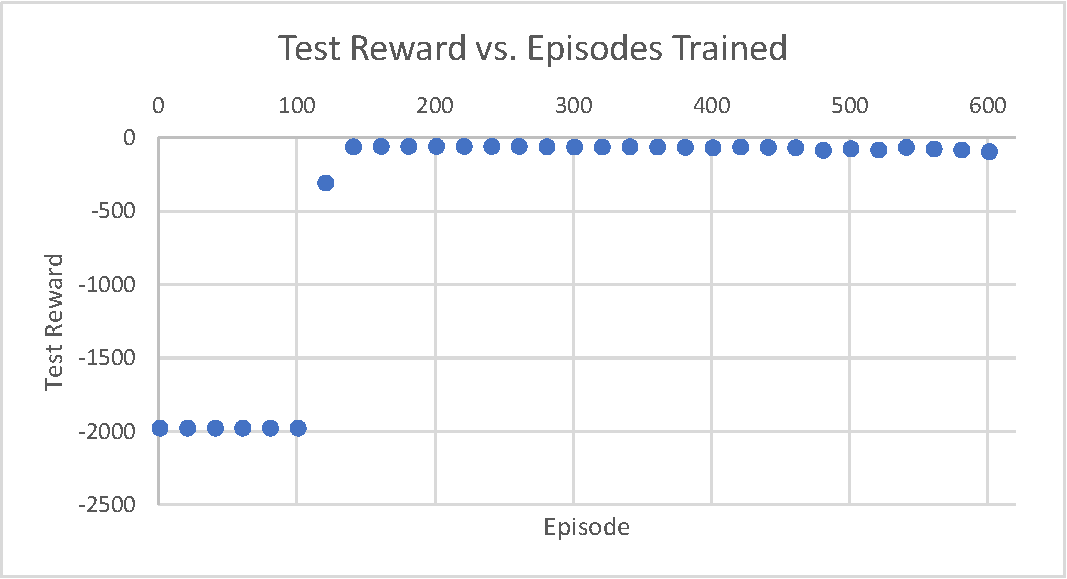
\includegraphics[width=6in, height=3.85in, keepaspectratio]{figures/train_figs/x_r.pdf}
	\caption{X Translation Test Reward} \label{fig:x_r}
\end{figure}
\begin{figure}[H]
	\centering
	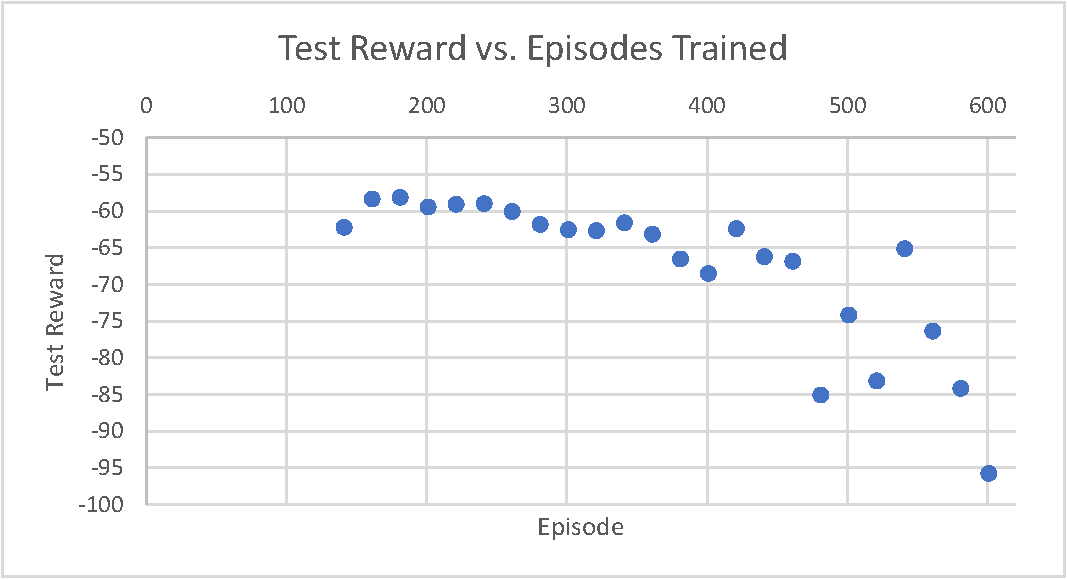
\includegraphics[width=6in, height=3.85in, keepaspectratio]{figures/train_figs/x_rzoom.pdf}
	\caption{X Translation Test Reward Zoomed} \label{fig:x_rzoom}
\end{figure}
\begin{figure}[H]
	\centering
	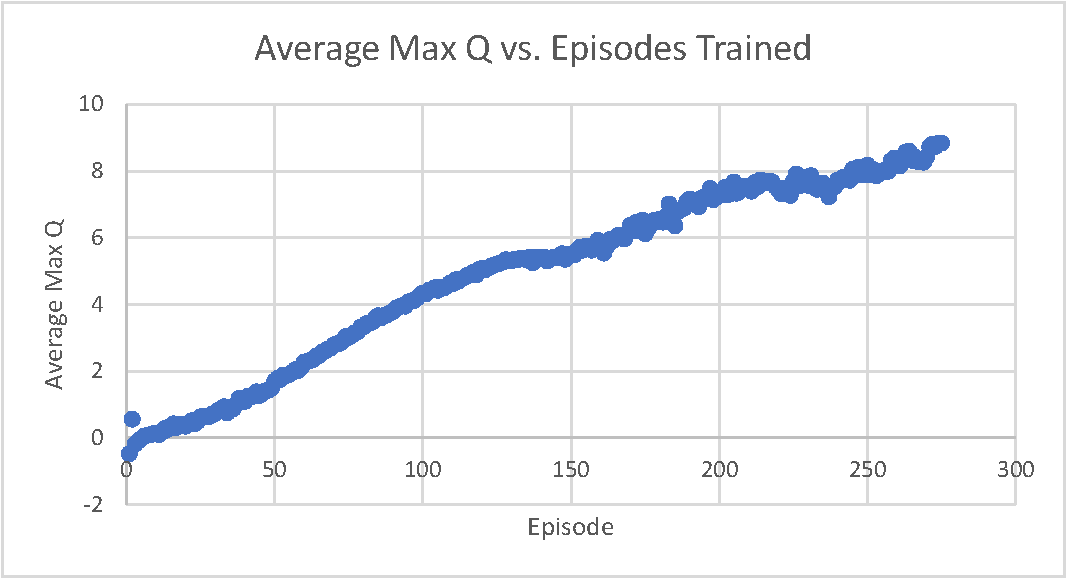
\includegraphics[width=6in, height=3.85in, keepaspectratio]{figures/train_figs/x_q.pdf}
	\caption{X Translation Network Average Max Q} \label{fig:x_q}
\end{figure}

Figure \ref{fig:x_perf} shows the action $u_x$, error from the set point, and reward versus time for eight episodes with different initial conditions after 161 episodes trained. Appendix \ref{appendix:x_perf} provides additional plots for different numbers of episodes trained. Regardless of the starting distance from the set point, the actor appears to drive the robot at maximum speed to reach the set point as quickly as possible since the positional error affects the reward most drastically. Soon after reaching the desired $x$ position, the action decays to zero.
\begin{figure}[H]
	\centering
	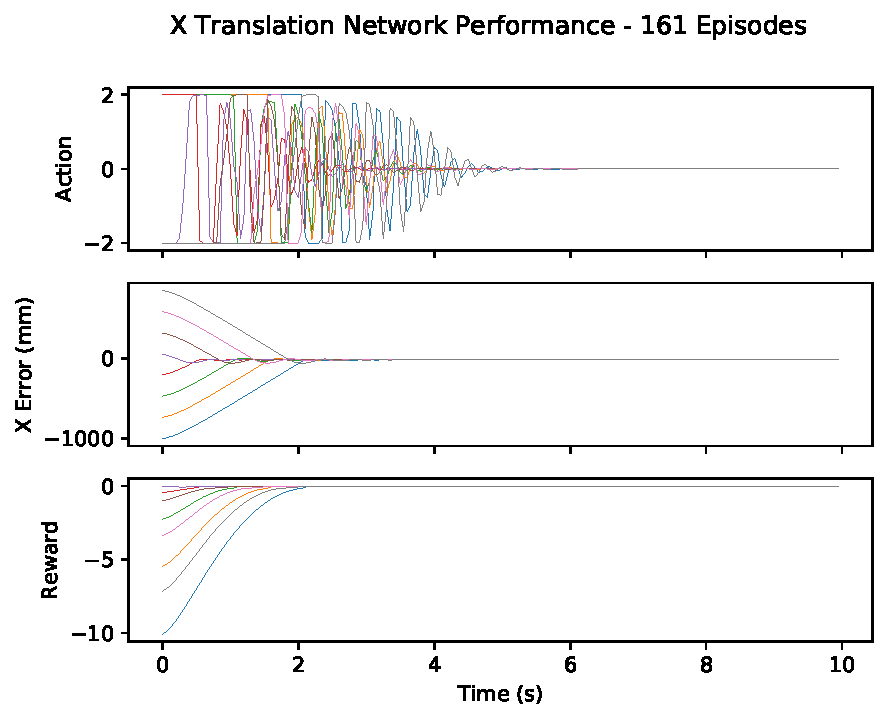
\includegraphics[width=6in, height=3.85in, keepaspectratio]{figures/train_figs/transx_transitions/1_161.pdf}
	\caption{X Translation Network Performance -- 161 Episodes}\label{fig:x_perf}
\end{figure}

Figure \ref{fig:x_actor_contour} displays a series of contour plots of the actor outputs as functions of the two inputs over different numbers of episodes trained where the color indicates the action $u_x$. The plots reveal the trained actor's output as highly polarized with only a sliver of low-valued $u_x$. Figure \ref{fig:x_critic_contour} shows a similar series of plots for the critic output. Since Q is a function of both the state and action, each point represents the highest Q-value among all actions at the particular state. The plot of Q follows intuition: the nearer the robot to the desired $x$ location, the greater the expected long-term reward.
\begin{figure}
	\begin{tabular}{cc}
		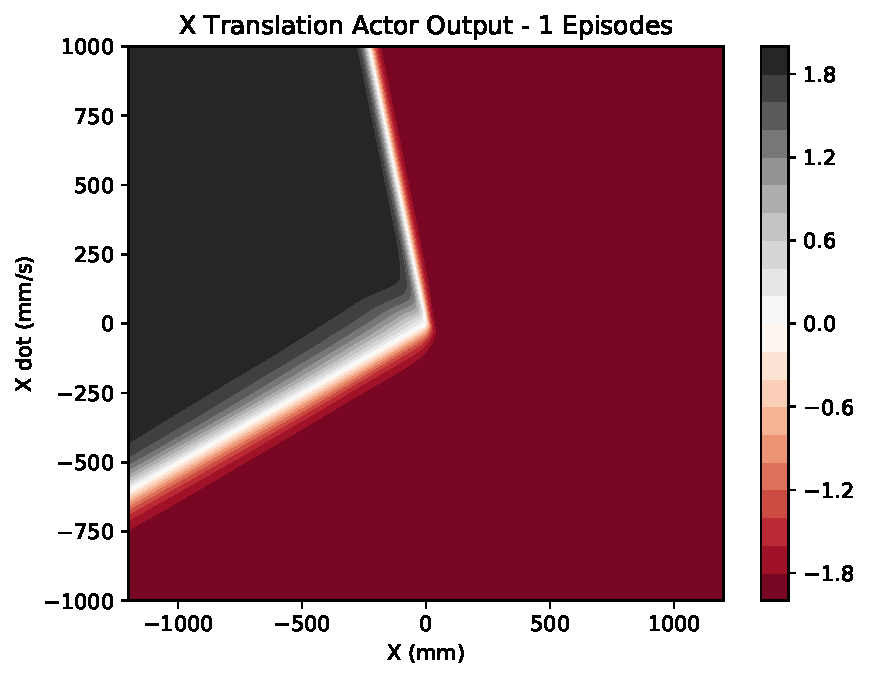
\includegraphics[width=65mm]{figures/train_figs/transx_actor/Actor1_1.pdf} &  
		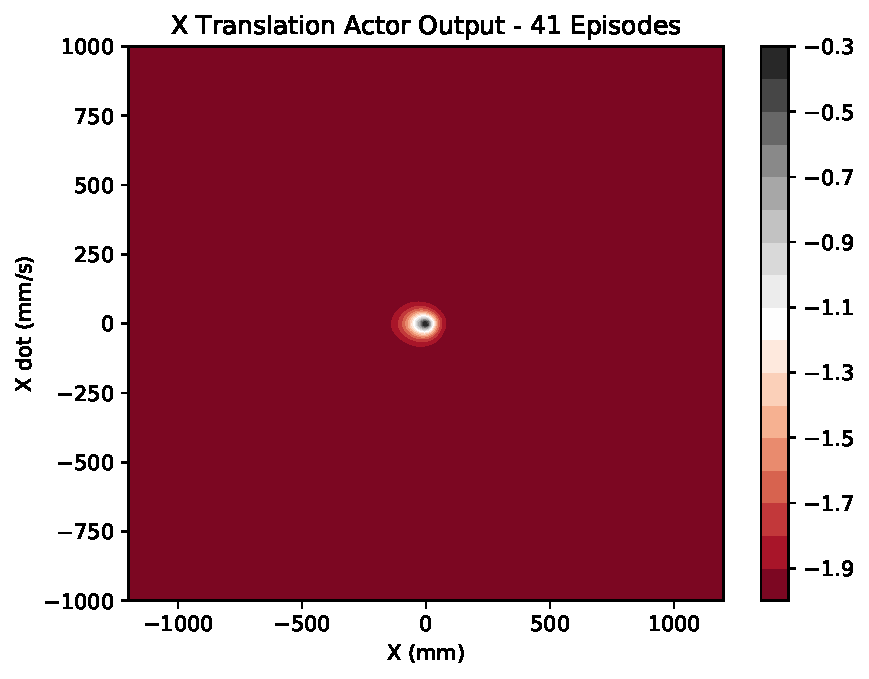
\includegraphics[width=65mm]{figures/train_figs/transx_actor/Actor1_41.pdf} \\
		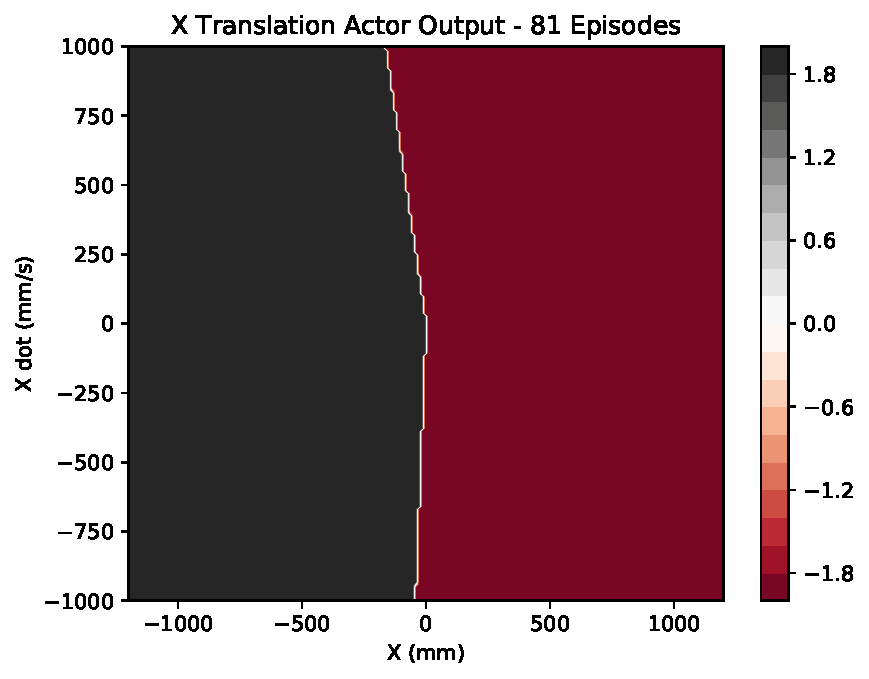
\includegraphics[width=65mm]{figures/train_figs/transx_actor/Actor1_81.pdf} &   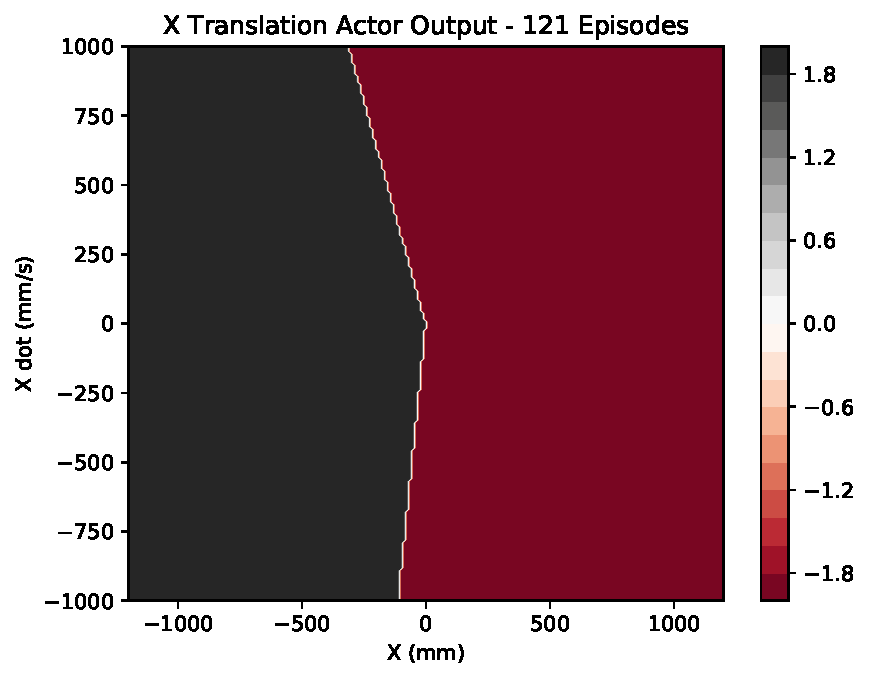
\includegraphics[width=65mm]{figures/train_figs/transx_actor/Actor1_121.pdf} \\
		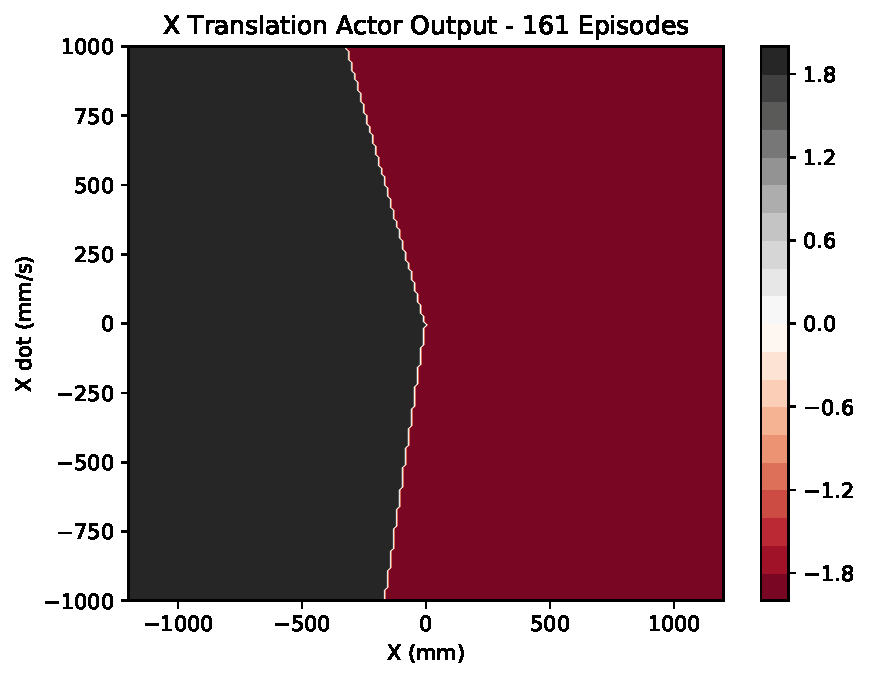
\includegraphics[width=65mm]{figures/train_figs/transx_actor/Actor1_161.pdf} &   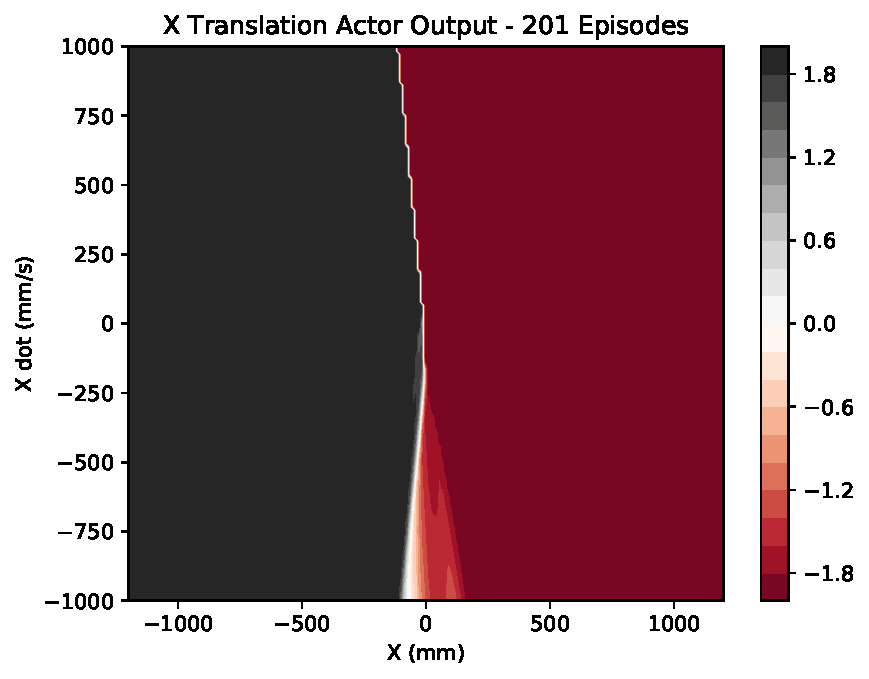
\includegraphics[width=65mm]{figures/train_figs/transx_actor/Actor1_201.pdf} \\
		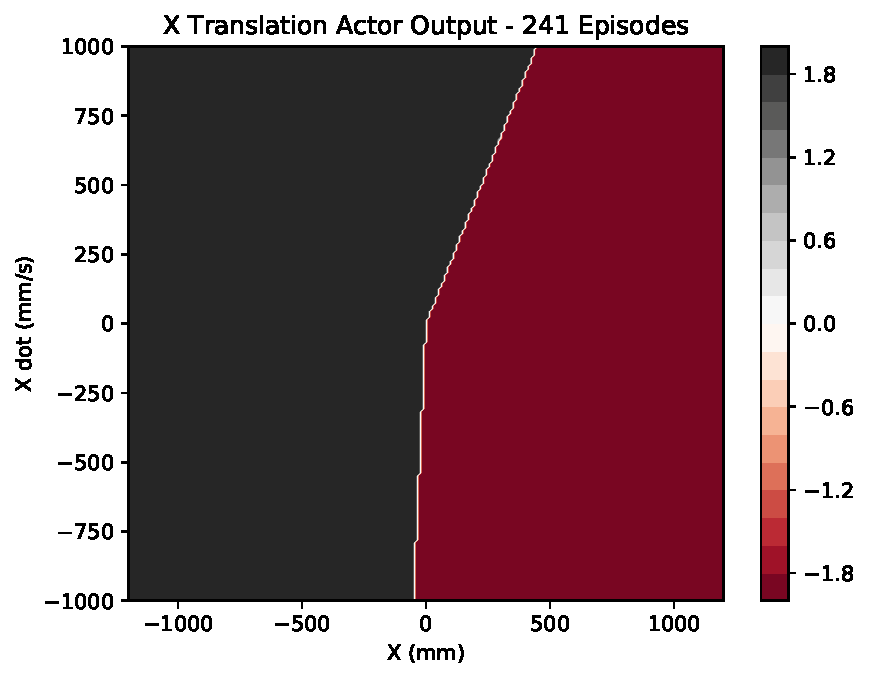
\includegraphics[width=65mm]{figures/train_figs/transx_actor/Actor1_241.pdf} &   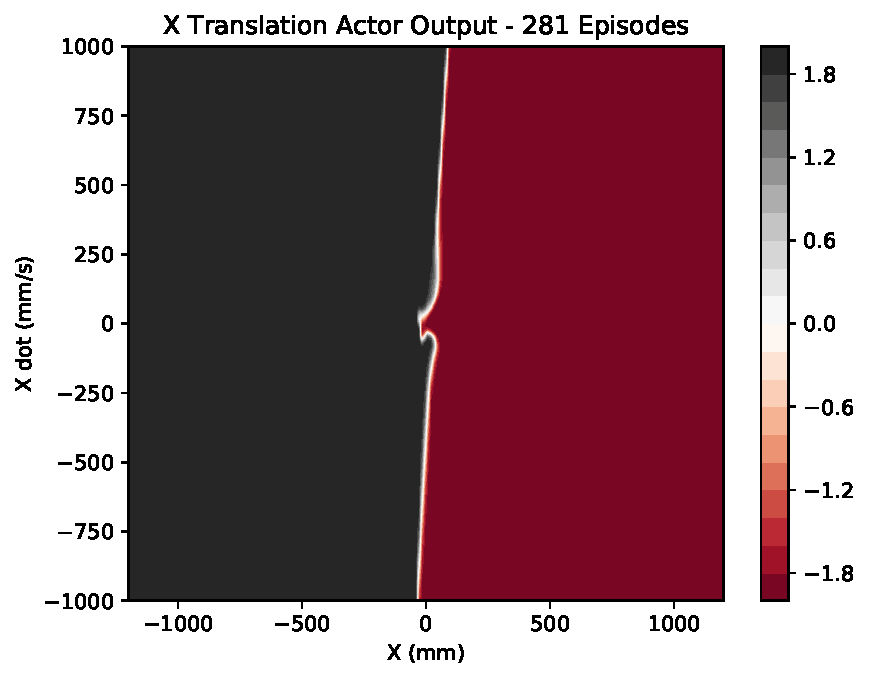
\includegraphics[width=65mm]{figures/train_figs/transx_actor/Actor1_281.pdf} \\
	\end{tabular}
	\caption{X Translation Actor Output Progression}\label{fig:x_actor_contour}
\end{figure}
\begin{figure}
	\begin{tabular}{cc}
		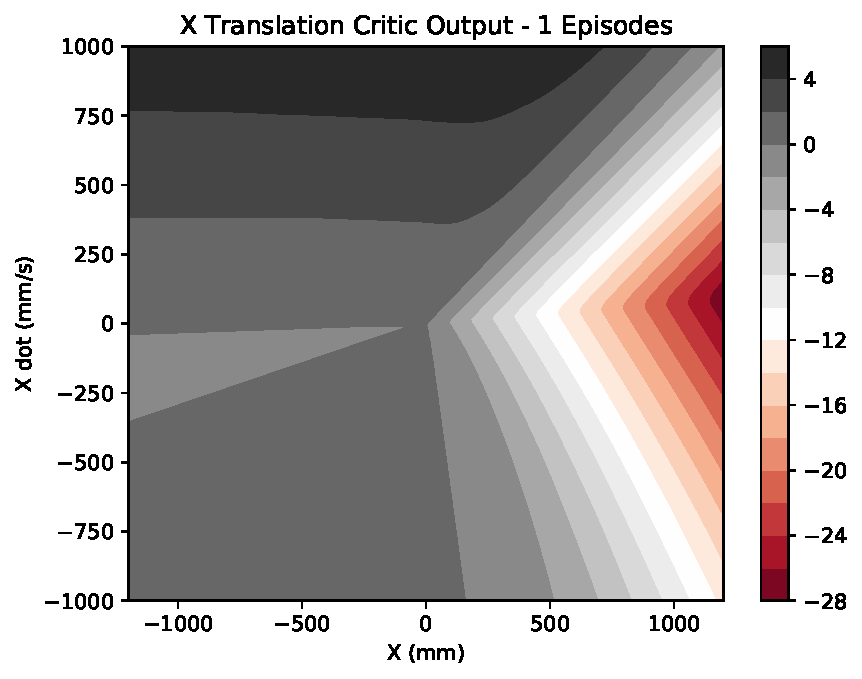
\includegraphics[width=65mm]{figures/train_figs/transx_critic/Critic1_1.pdf} &  
		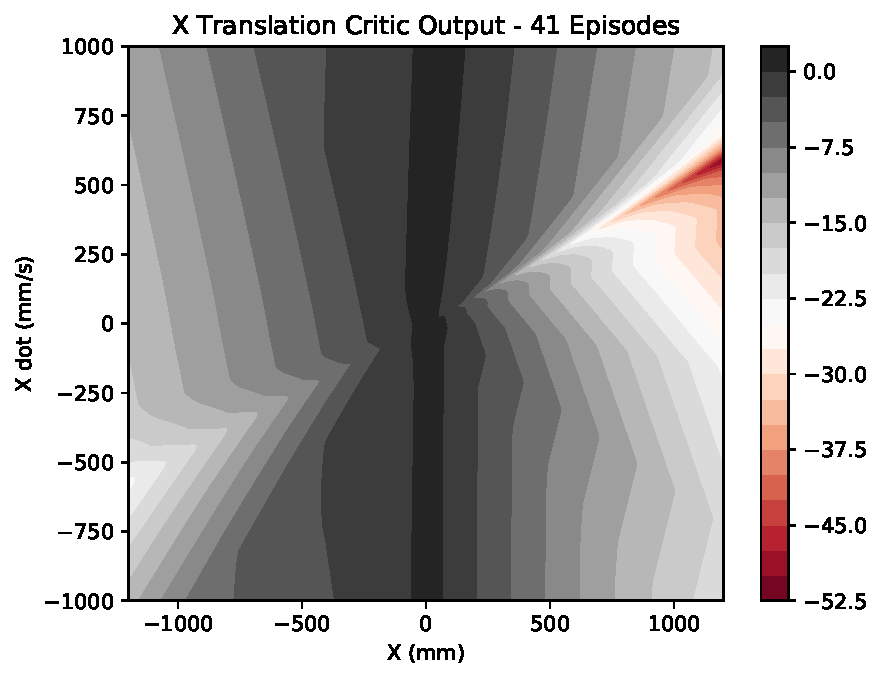
\includegraphics[width=65mm]{figures/train_figs/transx_critic/Critic1_41.pdf} \\
		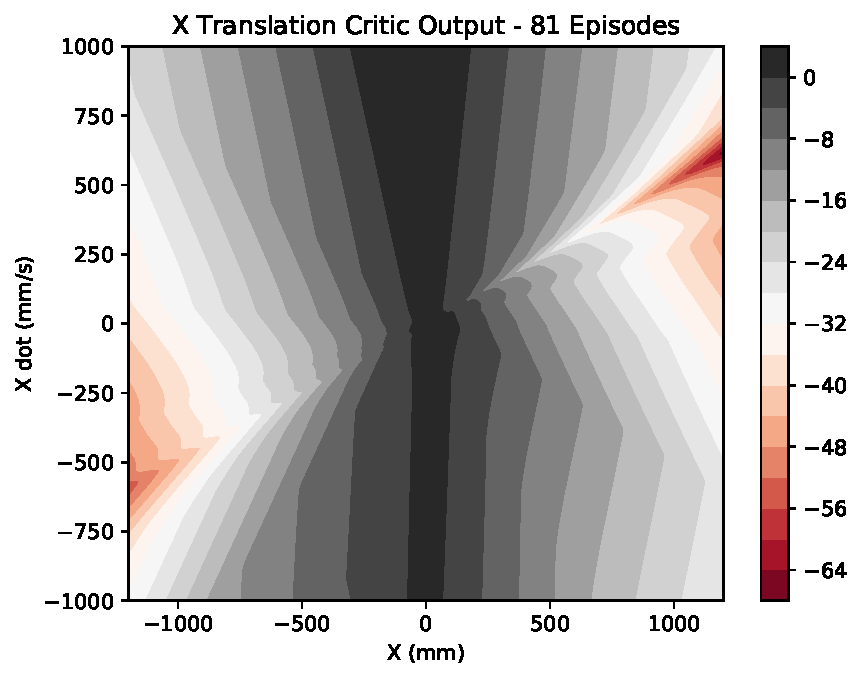
\includegraphics[width=65mm]{figures/train_figs/transx_critic/Critic1_81.pdf} &   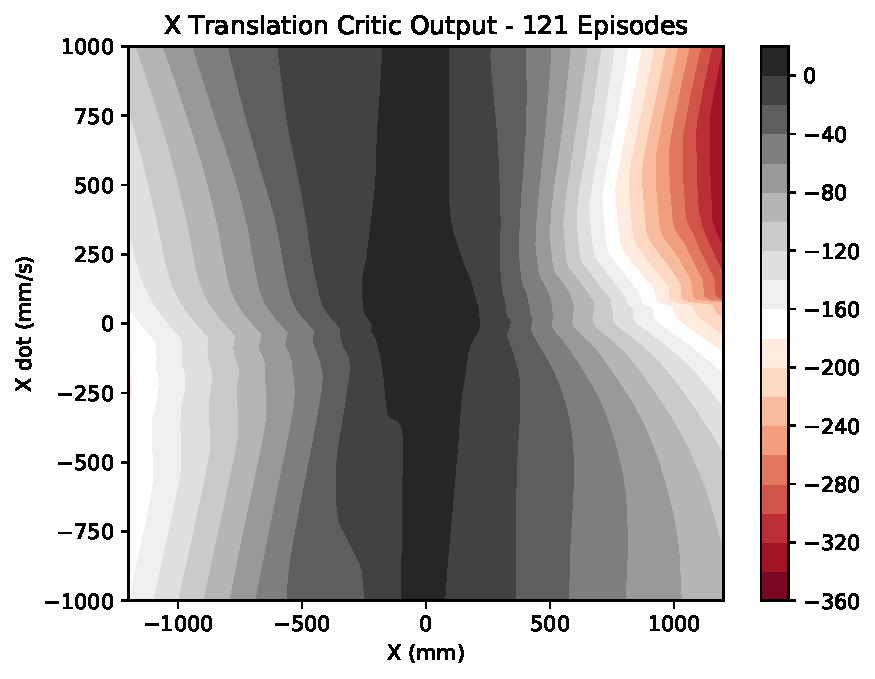
\includegraphics[width=65mm]{figures/train_figs/transx_critic/Critic1_121.pdf} \\
		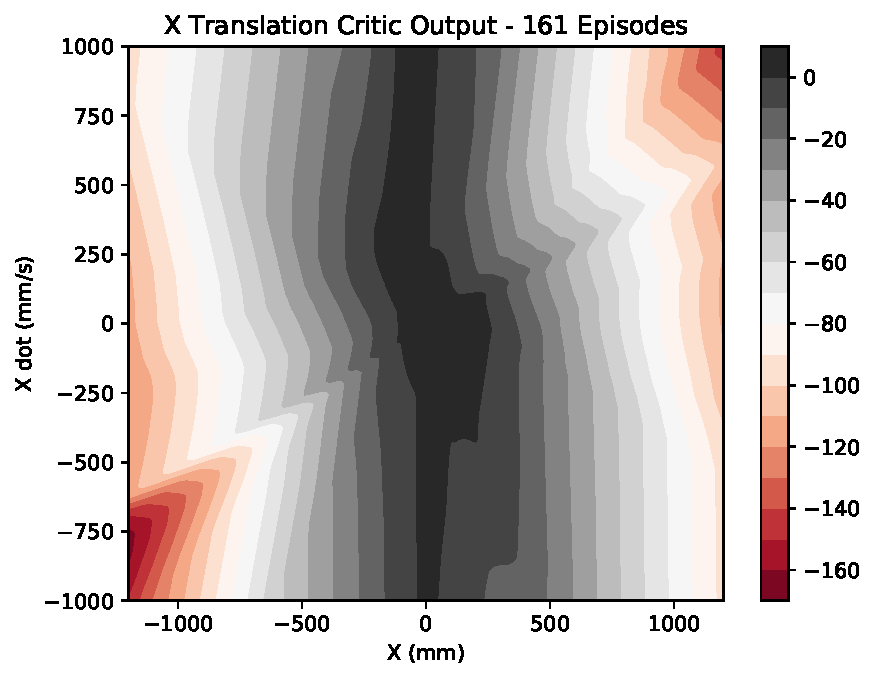
\includegraphics[width=65mm]{figures/train_figs/transx_critic/Critic1_161.pdf} &   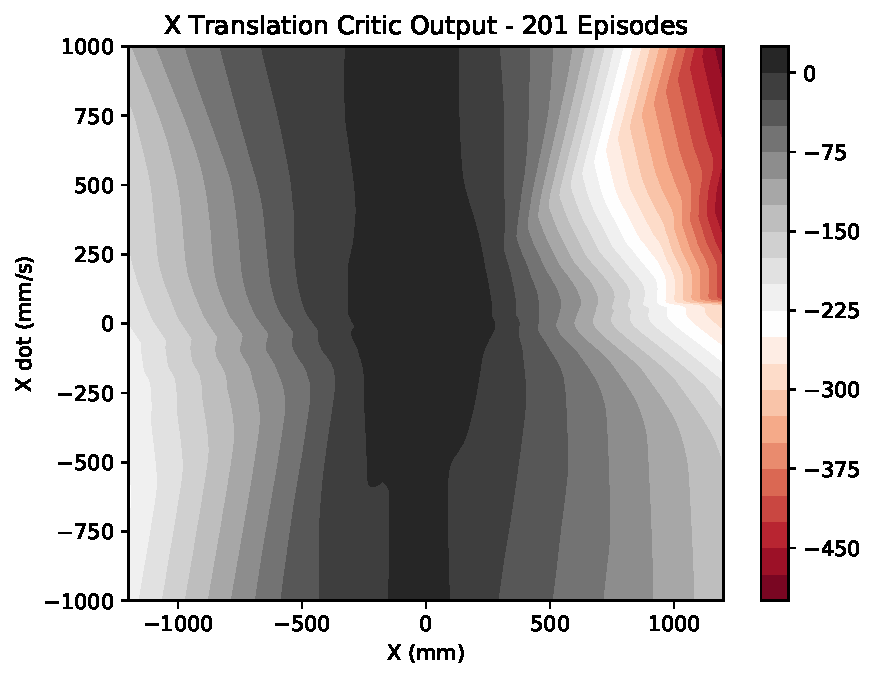
\includegraphics[width=65mm]{figures/train_figs/transx_critic/Critic1_201.pdf} \\
		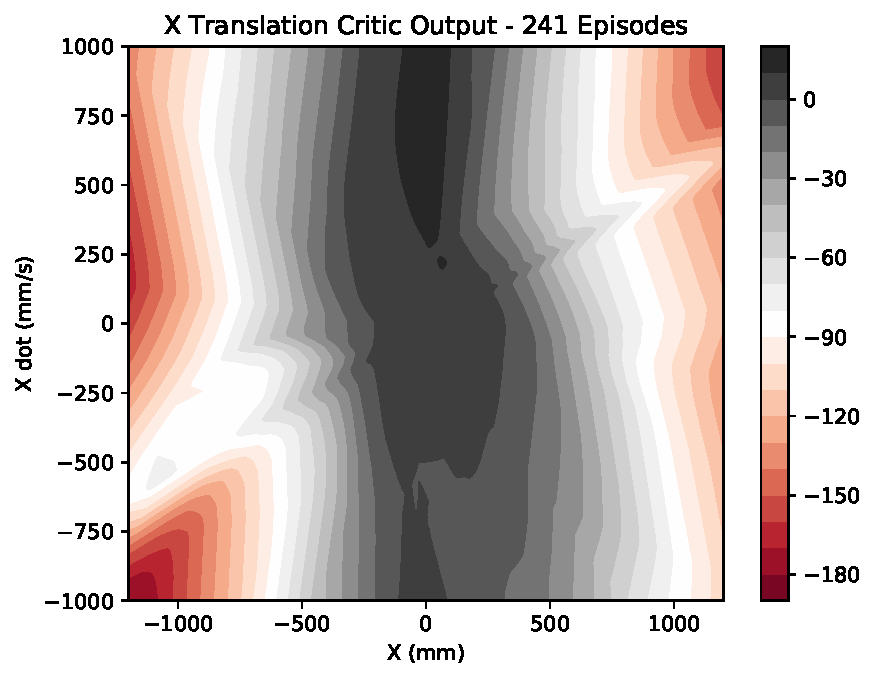
\includegraphics[width=65mm]{figures/train_figs/transx_critic/Critic1_241.pdf} &   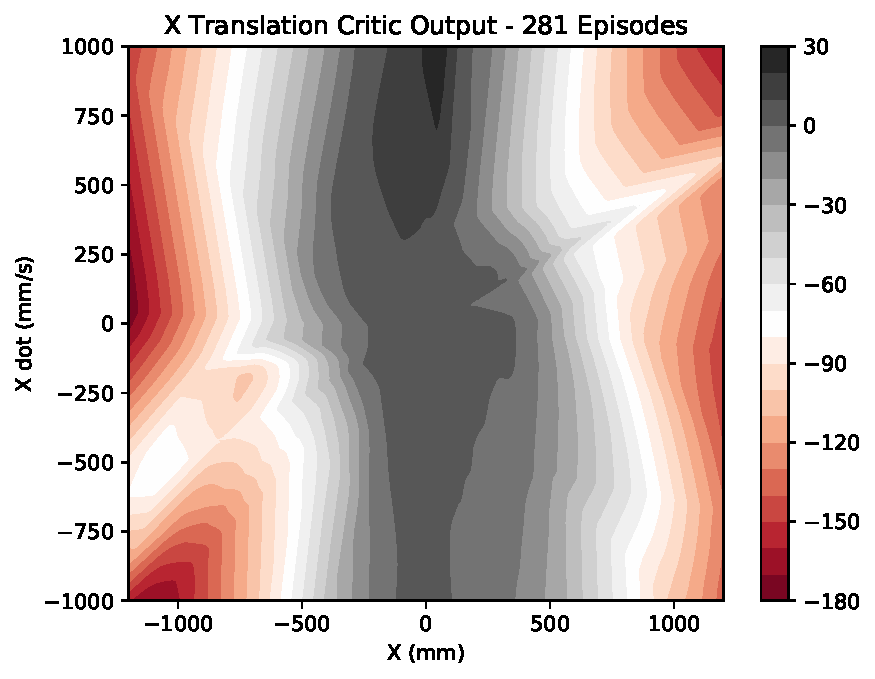
\includegraphics[width=65mm]{figures/train_figs/transx_critic/Critic1_281.pdf} \\
	\end{tabular}
	\caption{X Translation Critic Output Progression}\label{fig:x_critic_contour}
\end{figure}

\subsubsection{Y Translation Network}
The $y$ translation network is nearly identical to the $x$ translation but with a variable change so refer to the above for details. Figures \ref{fig:y_r} through \ref{fig:y_q} contain plots equivalent to those shown for the $x$ translation network. The test reward shows the same pattern of low test reward followed by a steep climb to a plateau. The jump in test reward aligns with the jump in average max Q at episode 161. The network also suffers from a decline in test reward from over training.
\begin{figure}[H]
	\centering
	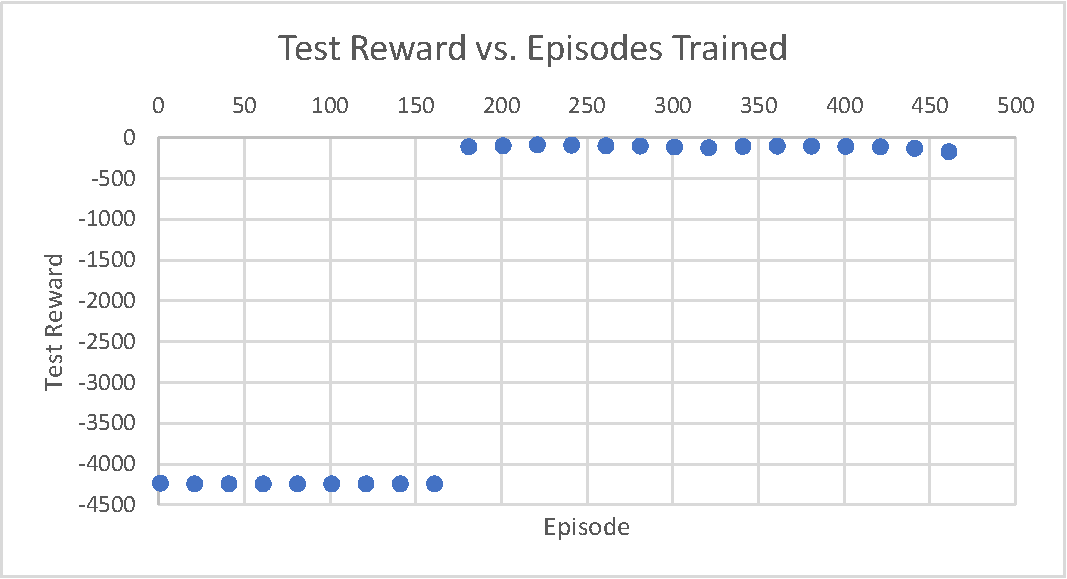
\includegraphics[width=6in, height=3.85in, keepaspectratio]{figures/train_figs/y_r.pdf}
	\caption{Y Translation Test Reward} \label{fig:y_r}
\end{figure}
\begin{figure}[H]
	\centering
	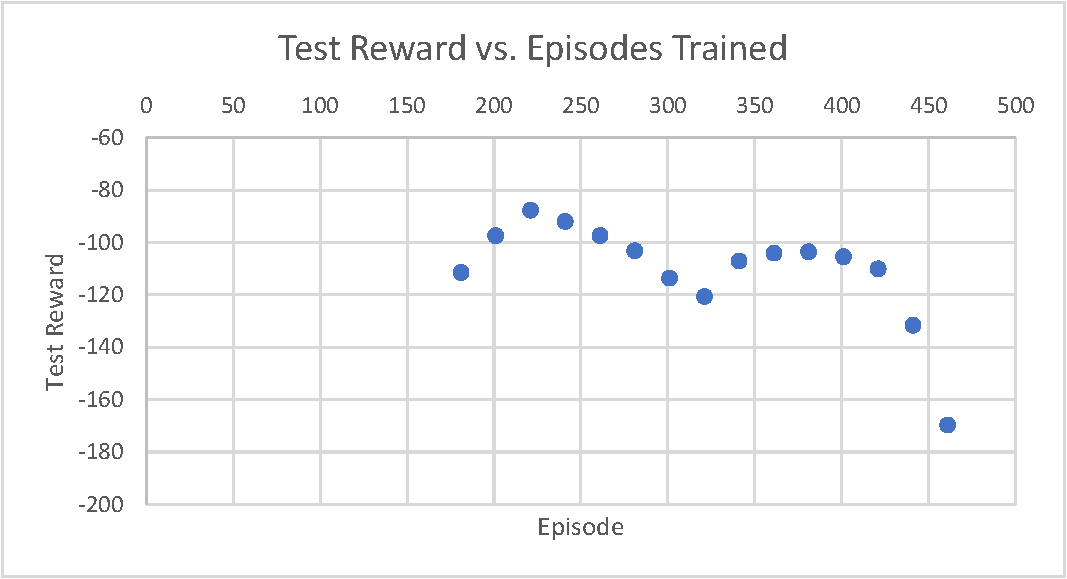
\includegraphics[width=6in, height=3.85in, keepaspectratio]{figures/train_figs/y_rzoom.pdf}
	\caption{Y Translation Test Reward Zoomed} \label{fig:y_rzoom}
\end{figure}
\begin{figure}[H]
	\centering
	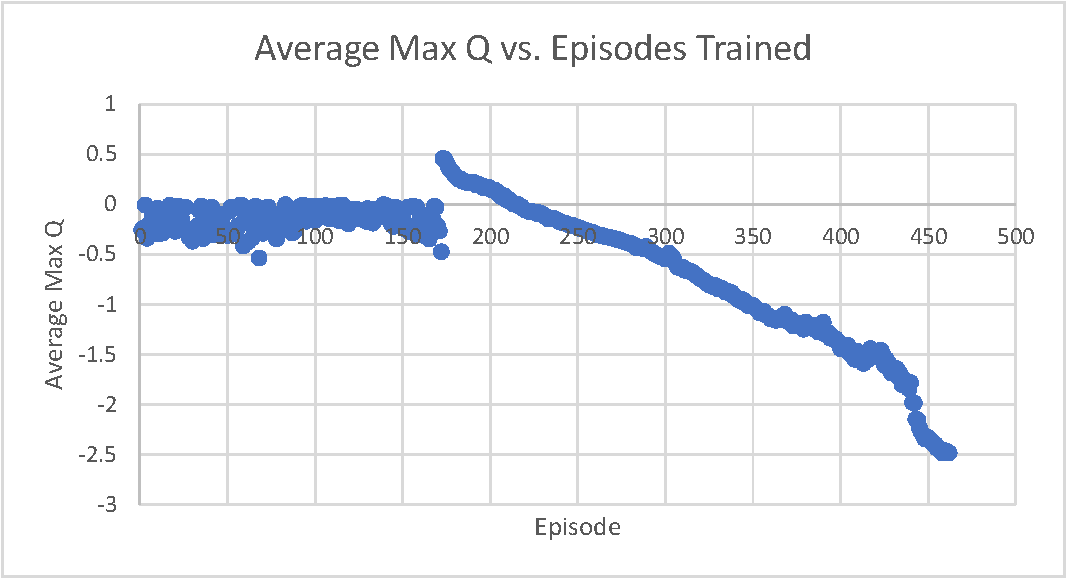
\includegraphics[width=6in, height=3.85in, keepaspectratio]{figures/train_figs/y_q.pdf}
	\caption{Y Translation Network Average Max Q} \label{fig:y_q}
\end{figure}

Figure \ref{fig:y_perf} displays the actor's transient response from eight different initial starting points after 221 episodes trained. Appendix \ref{appendix:y_perf} contains additional plots for other episodes trained. The robot reaches the set point with a small overshoot, and the action decays to zero as desired, indicating a successful policy.
\begin{figure}[H]
	\centering
	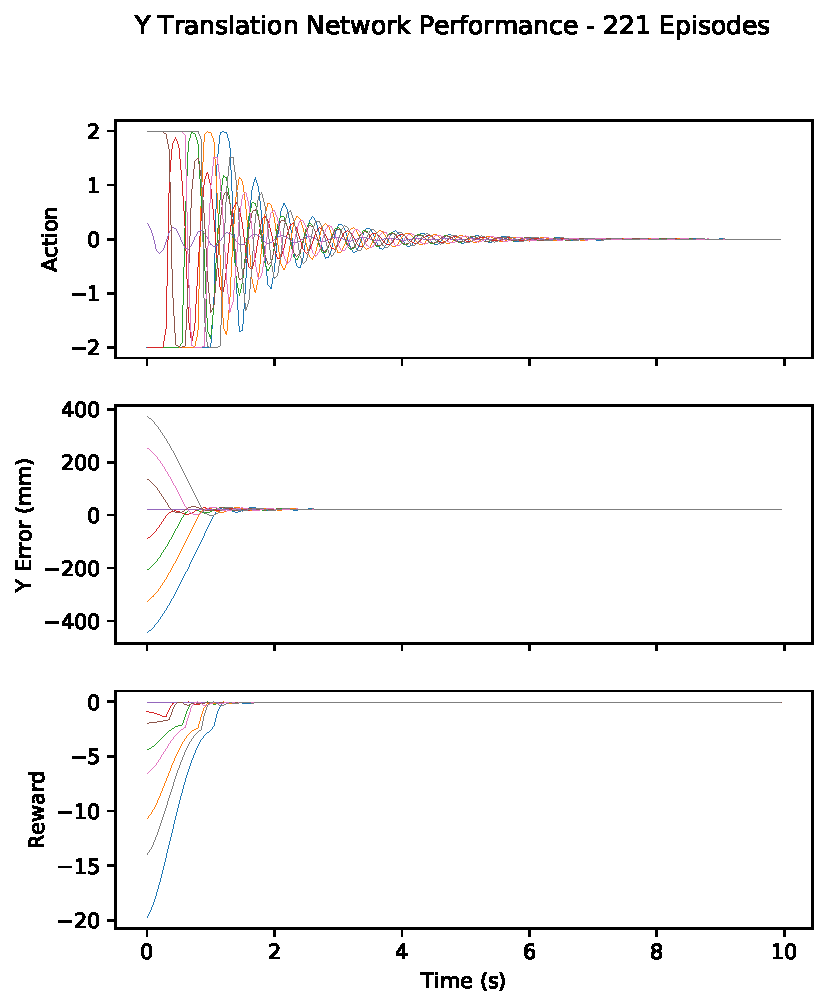
\includegraphics[width=6in, height=6in, keepaspectratio]{figures/train_figs/transy_transitions/2_221.pdf}
	\caption{Y Translation Network Performance -- 221 Episodes}\label{fig:y_perf}
\end{figure}

Figures \ref{fig:y_actor_contour} and \ref{fig:y_critic_contour} show the actor and critic contour plots, respectively. As expected, the contours are highly reminiscent of those for the $x$ translation network.
\begin{figure}[H]
	\begin{tabular}{cc}
		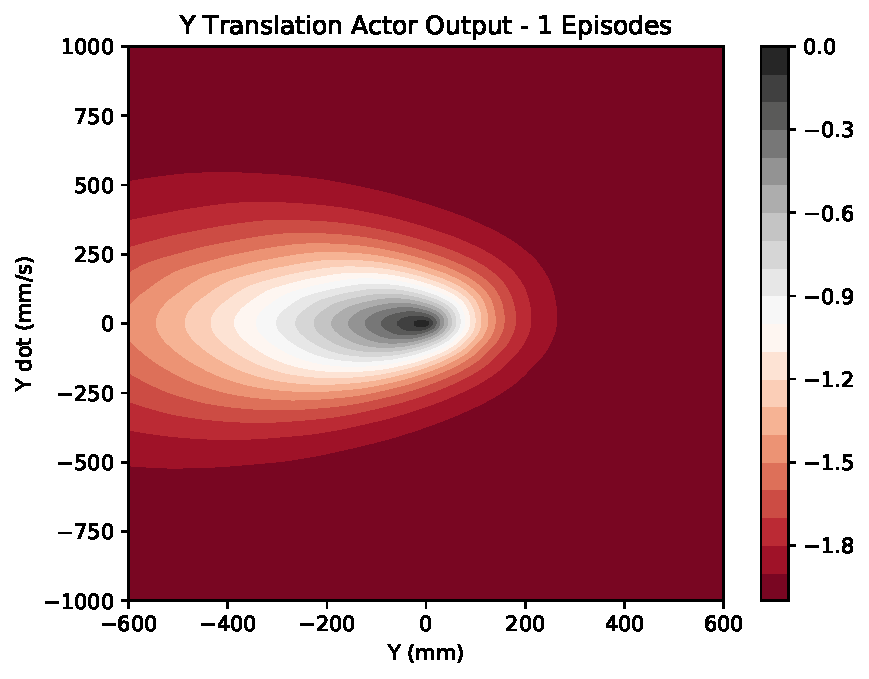
\includegraphics[width=65mm]{figures/train_figs/transy_actor/Actor2_1.pdf} &  
		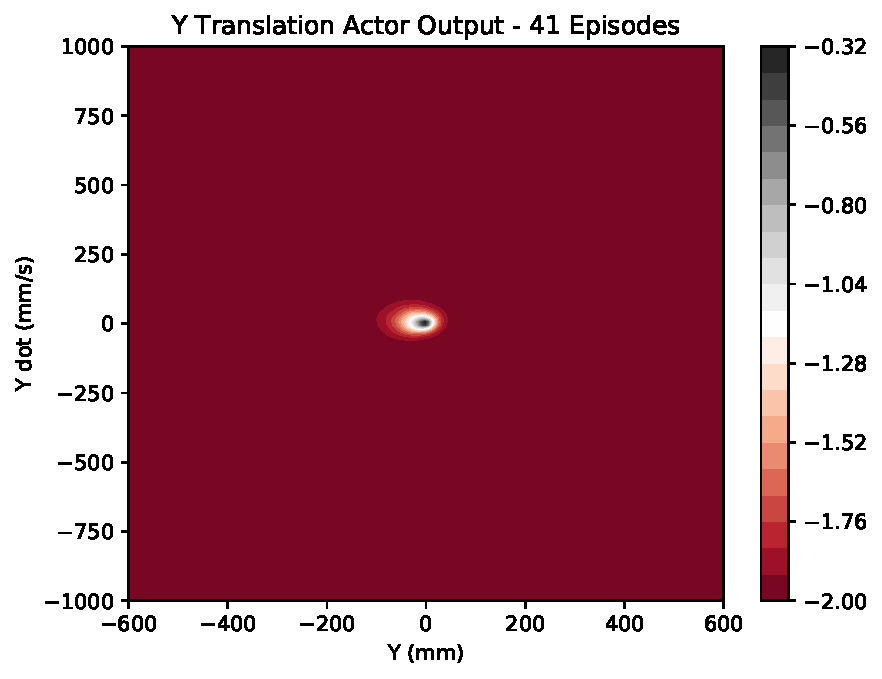
\includegraphics[width=65mm]{figures/train_figs/transy_actor/Actor2_41.pdf} \\
		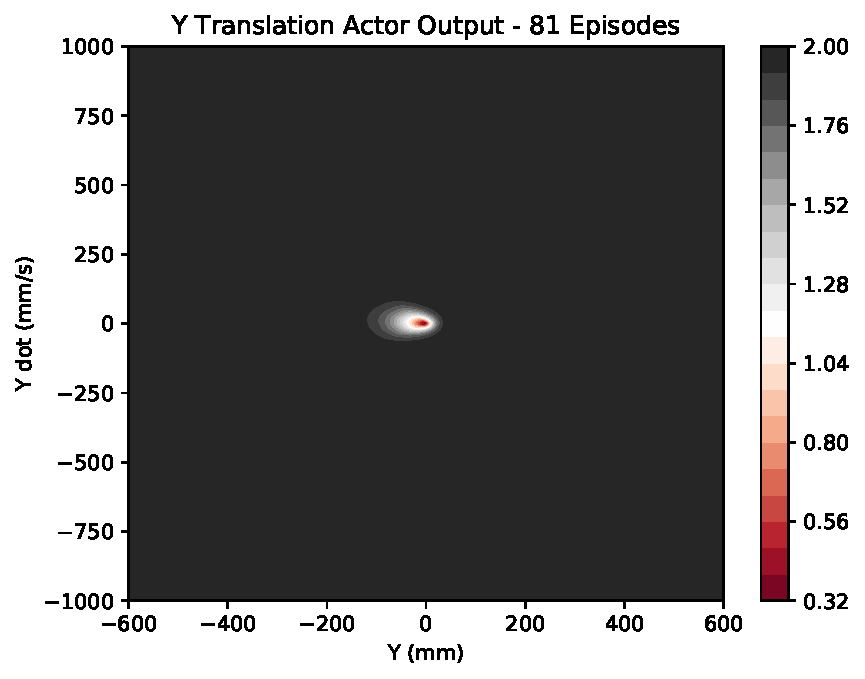
\includegraphics[width=65mm]{figures/train_figs/transy_actor/Actor2_81.pdf} &   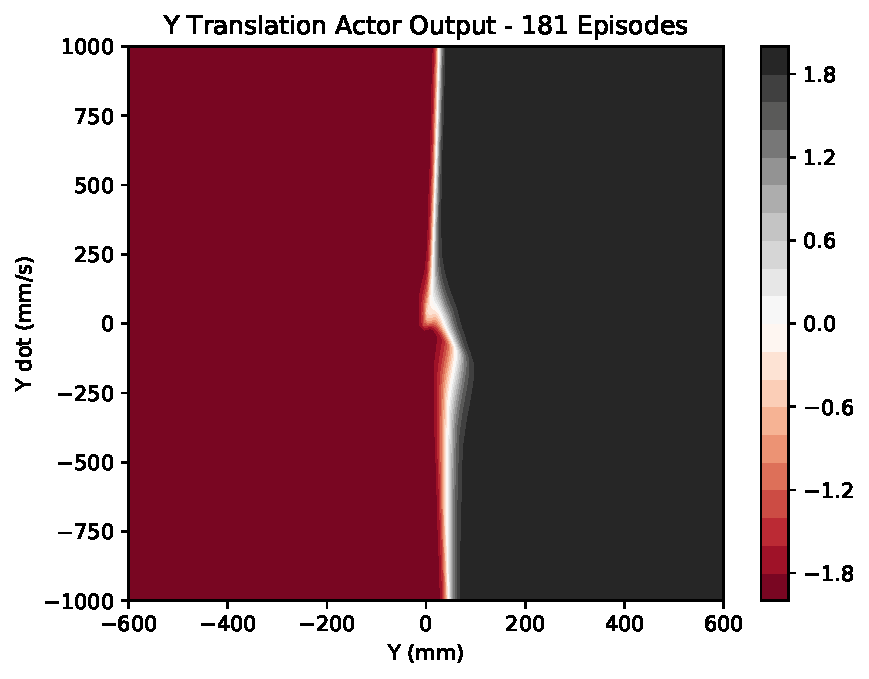
\includegraphics[width=65mm]{figures/train_figs/transy_actor/Actor2_181.pdf} \\
		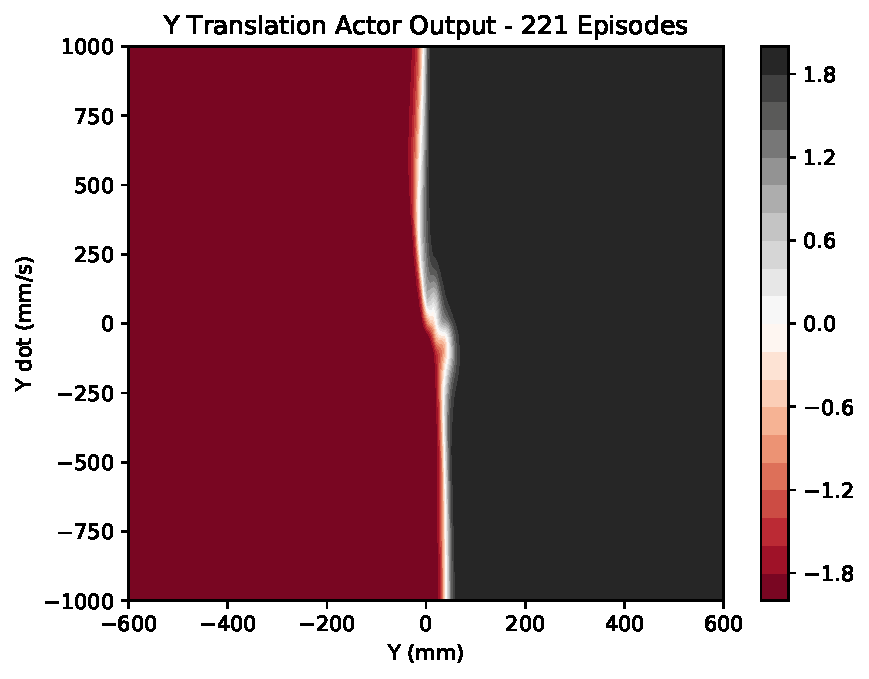
\includegraphics[width=65mm]{figures/train_figs/transy_actor/Actor2_221.pdf} &   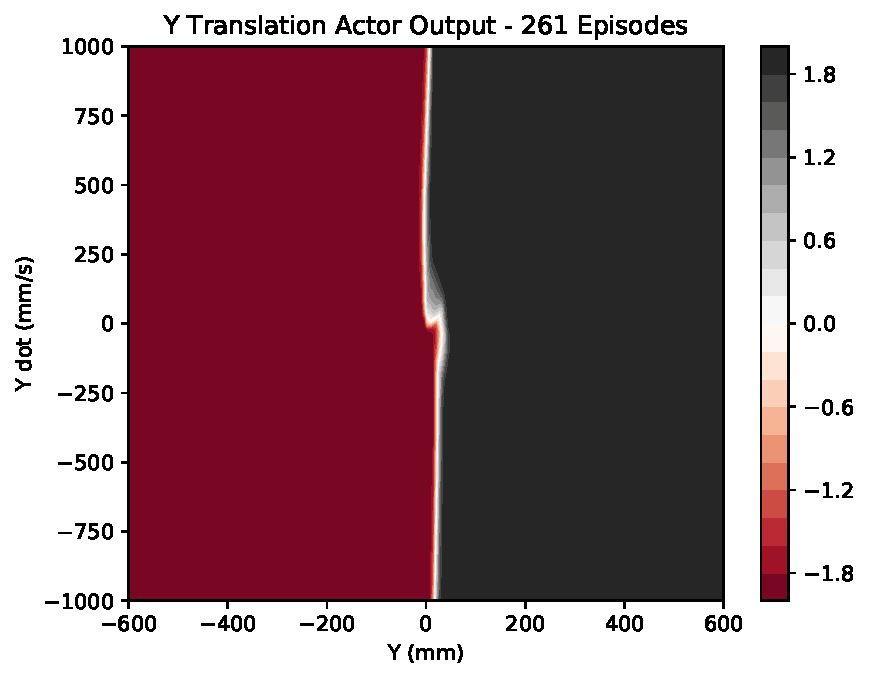
\includegraphics[width=65mm]{figures/train_figs/transy_actor/Actor2_261.pdf} \\
		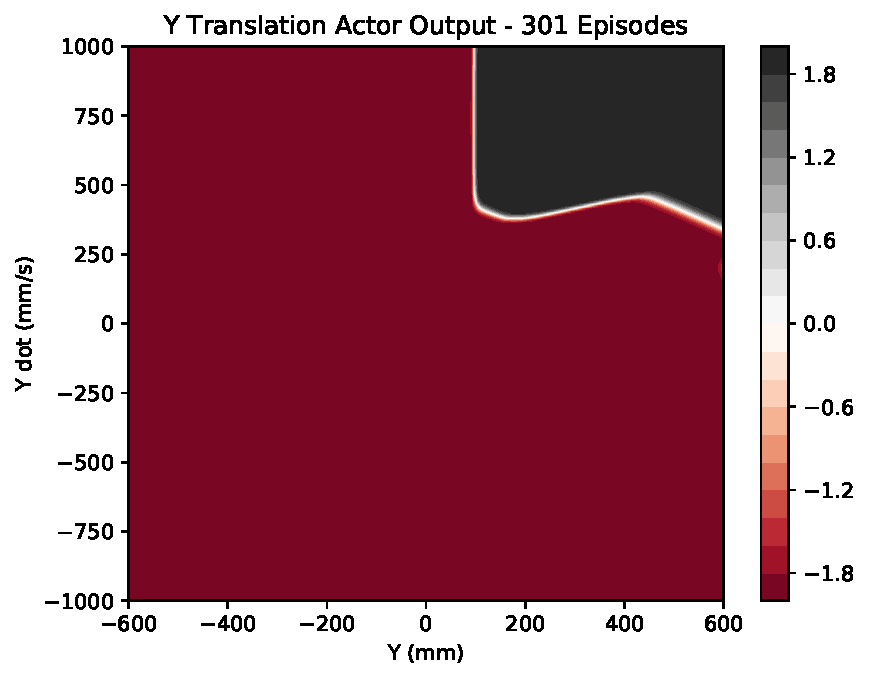
\includegraphics[width=65mm]{figures/train_figs/transy_actor/Actor2_301.pdf} &   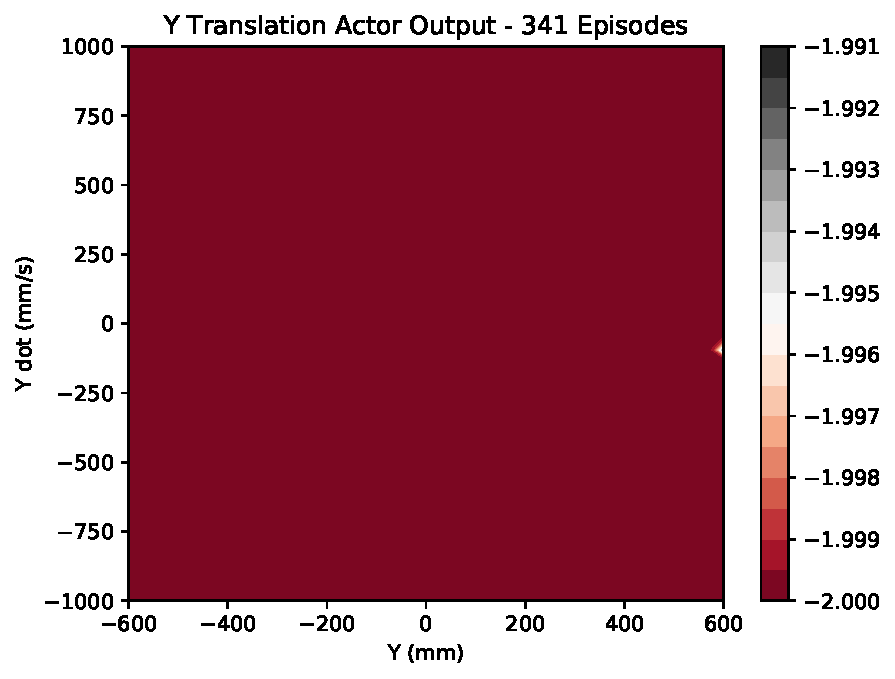
\includegraphics[width=65mm]{figures/train_figs/transy_actor/Actor2_341.pdf} \\
	\end{tabular}
	\caption{Y Translation Actor Output Progression}\label{fig:y_actor_contour}
\end{figure}
\begin{figure}[H]
	\begin{tabular}{cc}
		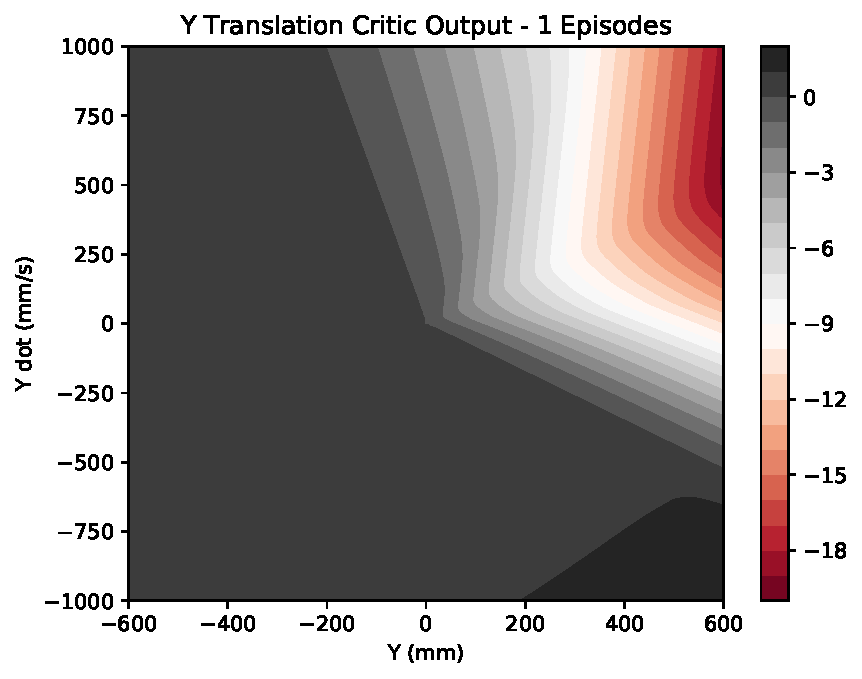
\includegraphics[width=65mm]{figures/train_figs/transy_critic/Critic2_1.pdf} &  
		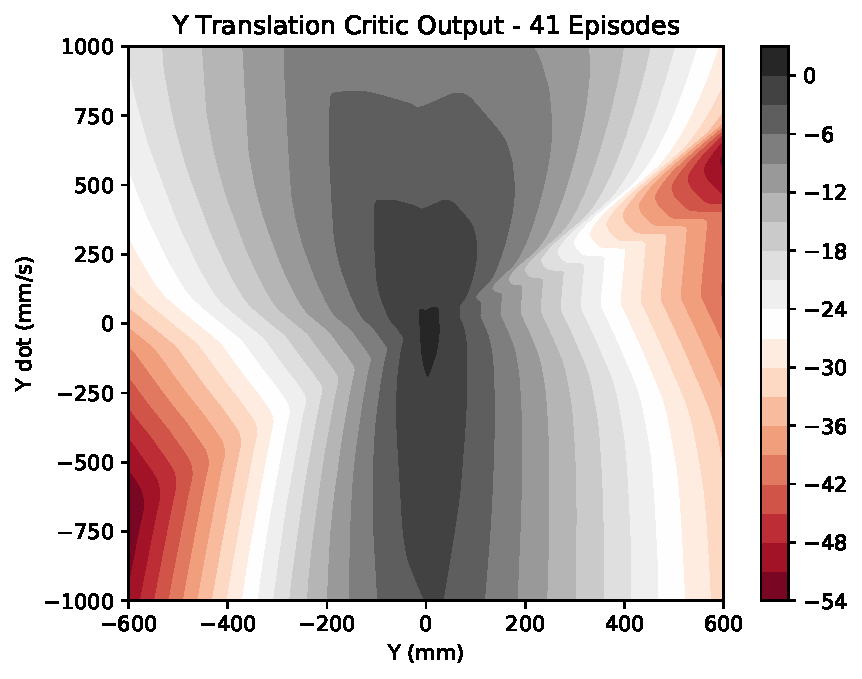
\includegraphics[width=65mm]{figures/train_figs/transy_critic/Critic2_41.pdf} \\
		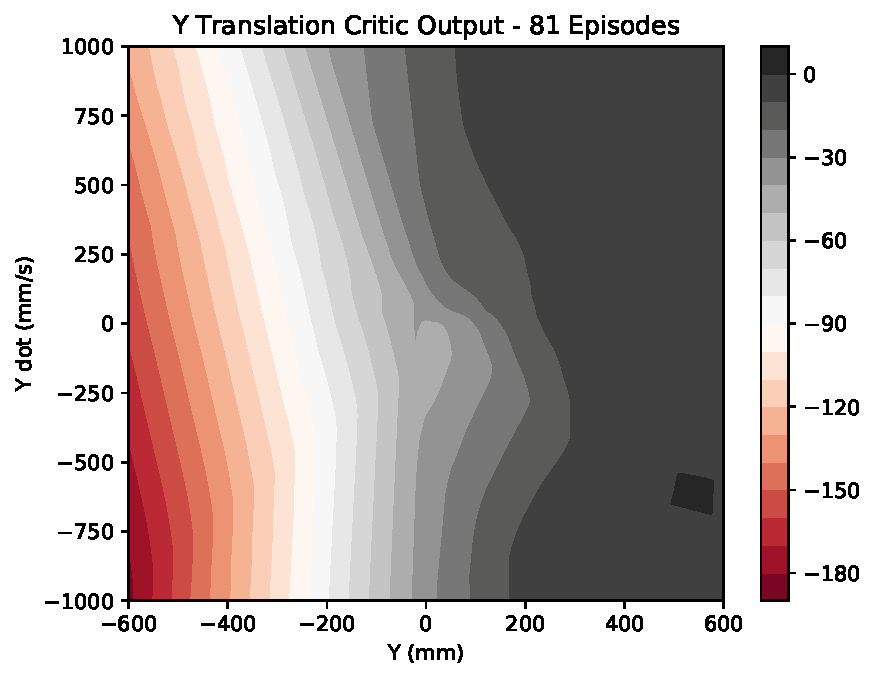
\includegraphics[width=65mm]{figures/train_figs/transy_critic/Critic2_81.pdf} &   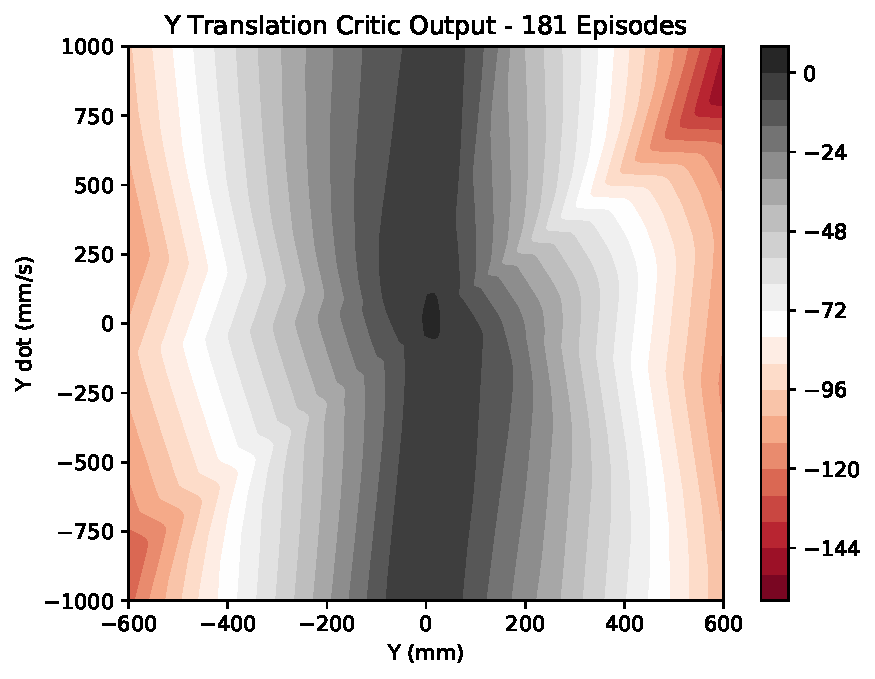
\includegraphics[width=65mm]{figures/train_figs/transy_critic/Critic2_181.pdf} \\
		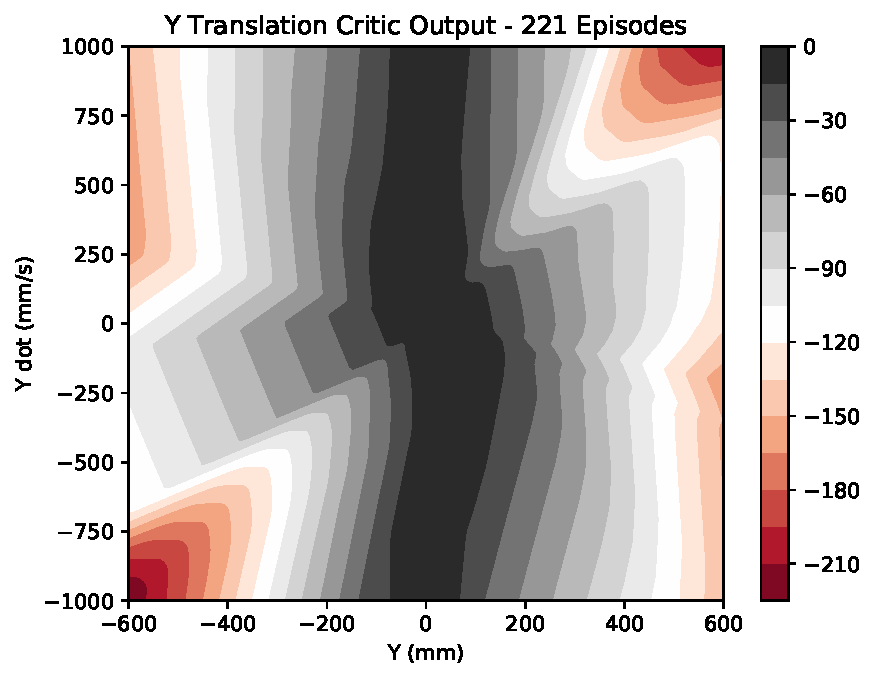
\includegraphics[width=65mm]{figures/train_figs/transy_critic/Critic2_221.pdf} &   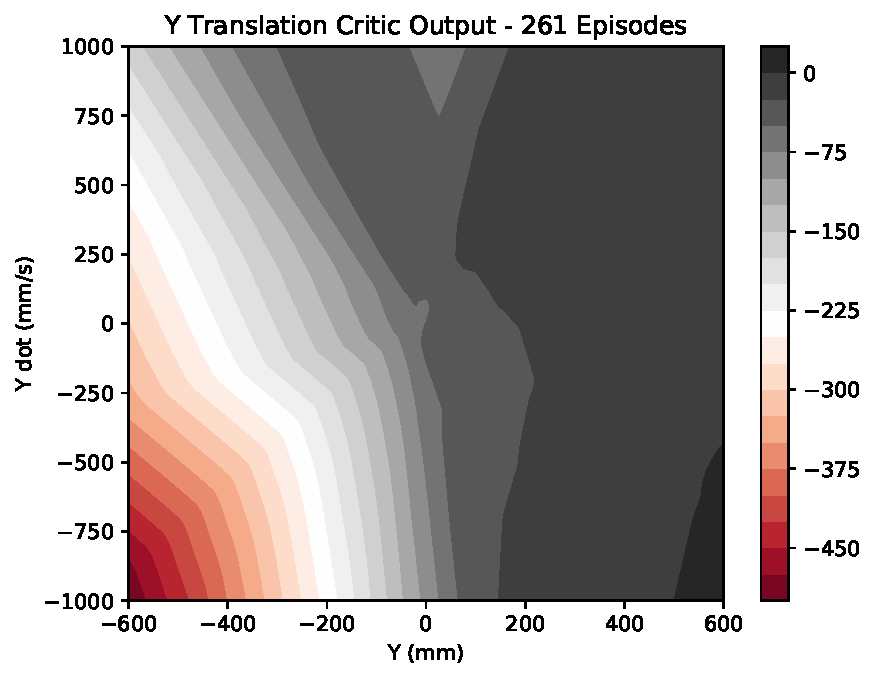
\includegraphics[width=65mm]{figures/train_figs/transy_critic/Critic2_261.pdf} \\
		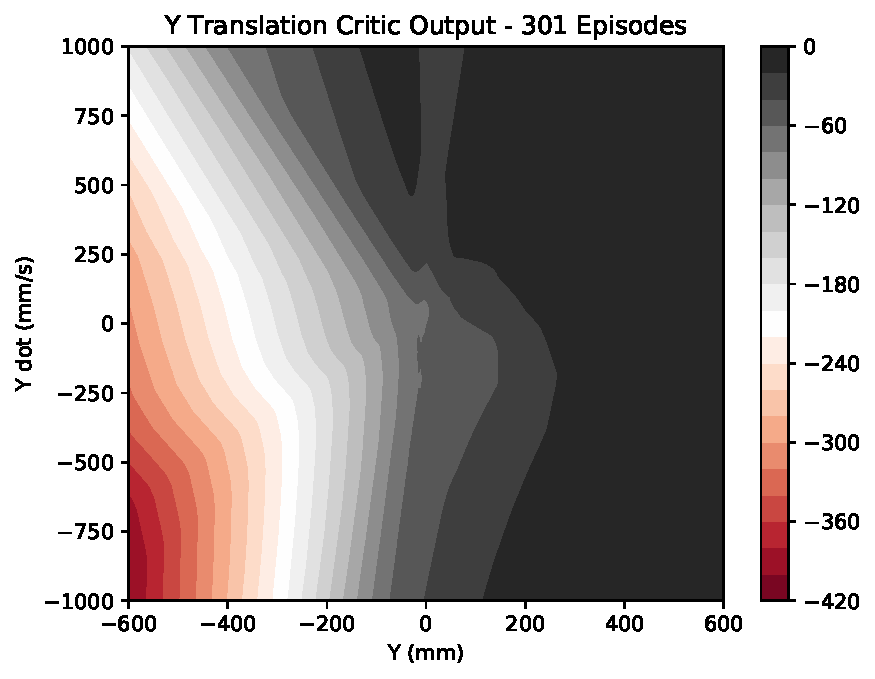
\includegraphics[width=65mm]{figures/train_figs/transy_critic/Critic2_301.pdf} &   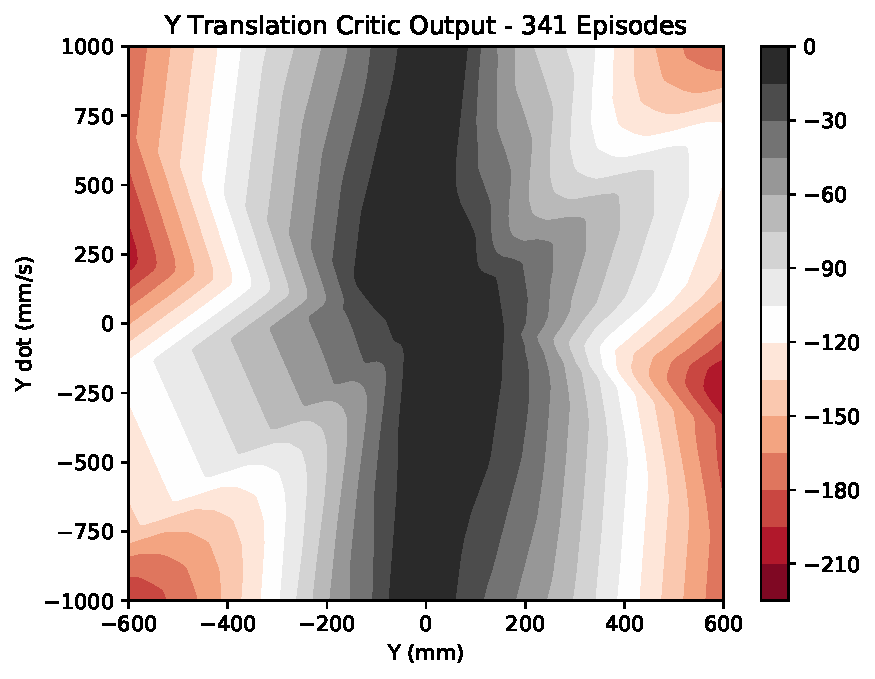
\includegraphics[width=65mm]{figures/train_figs/transy_critic/Critic2_341.pdf} \\
	\end{tabular}
	\caption{Y Translation Critic Output Progression}\label{fig:y_critic_contour}
\end{figure}

\subsubsection{Rotation Network}
The angle network receives the robot's angle error as $\text{cos}(\theta-\theta_{desired})$ and $\text{sin}(\theta-\theta_{desired})$ as well as the rotational velocity $\dot{\theta}$ and outputs $u_\theta$. The reward is calculated as shown in Equation \ref{eq:angle_reward} where the $\text{norm}()$ function normalizes the angle to between $-\pi$ and $+\pi$.
\begin{equation}
r = -1.0(\text{norm}(\theta)-\text{norm}(\theta_{desired}))^2-0.1\dot{\theta}^2-0.001u_\theta^2
\label{eq:angle_reward}
\end{equation}

Figures \ref{fig:angle_r} and \ref{fig:angle_rzoom} show test reward progress. The rotation network learns faster than either the $x$ or $y$ actors, achieving a reasonably good policy after only 41 episodes of training, due to the cyclical nature of rotation. Even if the actor decides to constantly spin the robot in one direction, it passes the set point with each revolution, obtaining useful experiences near the desired angle. However, in the $x$ or $y$ translation case, a constant movement in one direction leads the robot away from the set point and eventually gets it stuck at a wall instead of gaining effective experiences.
\begin{figure}[H]
	\centering
	\includegraphics[width=6in, height=3.85in, keepaspectratio]{figures/train_figs/angle_r.pdf}
	\caption{Angle Test Reward} \label{fig:angle_r}
\end{figure}
\begin{figure}[H]
	\centering
	\includegraphics[width=6in, height=3.85in, keepaspectratio]{figures/train_figs/angle_rzoom.pdf}
	\caption{Angle Test Reward Zoomed} \label{fig:angle_rzoom}
\end{figure}
\begin{figure}[H]
	\centering
	\includegraphics[width=6in, height=3.85in, keepaspectratio]{figures/train_figs/angle_q.pdf}
	\caption{Angle Network Average Max Q} \label{fig:angle_q}
\end{figure}

As seen in Figure \ref{fig:angle_perf}, the rotation actor monotonically brings the robot to the desired angle with no overshoot and reduces the action to 0 afterwards. Appendix \ref{appendix:angle_perf} provides additional plots for different numbers of episodes trained. 
\begin{figure}[H]
	\centering
	\includegraphics[width=6in, height=3.85in, keepaspectratio]{figures/train_figs/angle_transitions/0_61.pdf}
	\caption{Angle Network Performance -- 61 Episodes}\label{fig:angle_perf}
\end{figure}

Figures \ref{fig:angle_actor_contour} and \ref{fig:angle_critic_contour} contain contour plots of the actor and critic outputs. As expected, the plots are periodic with respect to $\theta$. The actor contours take on a vaguely sinusoidal shape with only a thin sliver of area producing low action values, much like the other two networks. The critic network produces high Q values for states near the desired angle and low angular velocity.
\begin{figure}[H]
	\begin{tabular}{cc}
		\includegraphics[width=65mm]{figures/train_figs/angle_actor/Actor0_1.pdf} &  
		\includegraphics[width=65mm]{figures/train_figs/angle_actor/Actor0_21.pdf} \\
		\includegraphics[width=65mm]{figures/train_figs/angle_actor/Actor0_61.pdf} &   \includegraphics[width=65mm]{figures/train_figs/angle_actor/Actor0_81.pdf} \\
		\includegraphics[width=65mm]{figures/train_figs/angle_actor/Actor0_121.pdf} &   \includegraphics[width=65mm]{figures/train_figs/angle_actor/Actor0_161.pdf} \\
		\includegraphics[width=65mm]{figures/train_figs/angle_actor/Actor0_221.pdf} &   \includegraphics[width=65mm]{figures/train_figs/angle_actor/Actor0_301.pdf} \\
	\end{tabular}
	\caption{Angle Actor Output Progression}\label{fig:angle_actor_contour}
\end{figure}
\begin{figure}[H]
	\begin{tabular}{cc}
		\includegraphics[width=65mm]{figures/train_figs/angle_critic/Critic0_1.pdf} &  
		\includegraphics[width=65mm]{figures/train_figs/angle_critic/Critic0_21.pdf} \\
		\includegraphics[width=65mm]{figures/train_figs/angle_critic/Critic0_61.pdf} &   \includegraphics[width=65mm]{figures/train_figs/angle_critic/Critic0_81.pdf} \\
		\includegraphics[width=65mm]{figures/train_figs/angle_critic/Critic0_121.pdf} &   \includegraphics[width=65mm]{figures/train_figs/angle_critic/Critic0_161.pdf} \\
		\includegraphics[width=65mm]{figures/train_figs/angle_critic/Critic0_221.pdf} &   \includegraphics[width=65mm]{figures/train_figs/angle_critic/Critic0_301.pdf} \\
	\end{tabular}
	\caption{Angle Critic Output Progression}\label{fig:angle_critic_contour}
\end{figure}

\subsection{Three Actors Combined}
After the three networks were trained, the best iteration of each (determined as rapid settling time, low or no overshoot, and decaying action value) was combined. At each time step, each actor produces its respective control component which merge together using Equations \ref{eq:mecanum_v0} through \ref{eq:mecanum_v3} as described previously. Figure \ref{fig:three_actor_response} displays the response to eight varied initial states. Although the robot reaches the desired $x$, $y$, and $\theta$ position, it takes longer than in the individual tests above since the robot's movement is now divided amongst the three directions $x$, $y$, and $\theta$. The actions still decay to 0. 
\begin{figure}[H]
	\centering
	\includegraphics[width=6in, height=5in, keepaspectratio]{figures/three_actor_response.pdf}
	\caption{Combined Response} \label{fig:three_actor_response}
\end{figure}

\subsection{Single Actor Network}
Since single actor approach required reduced learning rates to prevent training instability, the network trained for substantially longer before achieving reasonable performance. Figures \ref{fig:all_r} and \ref{fig:all_rzoom} show that the learning ``jump'' lasts nearly 1,000 episodes versus 20-60 episodes in the three actor case. Notably, Figure \ref{fig:all_rzoom} shows that, on average, the test reward continues to very slightly increase with further training at a rate of 1.6 reward per 1,000 additional episodes trained. In Figure \ref{fig:all_q}, the average max Q overshoots the ideal maximum of 0 but settles to negative values with further training.
\begin{figure}[H]
	\includegraphics[width=6in, height=3.85in, keepaspectratio]{figures/train_figs/all_r.pdf}
	\caption{Training and Test Reward} \label{fig:all_r}
\end{figure}
\begin{figure}[H]
	\includegraphics[width=6in, height=3.85in, keepaspectratio]{figures/train_figs/all_rzoom.pdf}
	\caption{Training and Test Reward Zoomed} \label{fig:all_rzoom}
\end{figure}
\begin{figure}[H]
	\includegraphics[width=6in, height=3.85in, keepaspectratio]{figures/train_figs/all_q.pdf}
	\caption{Average Max Q} \label{fig:all_q}
\end{figure}

Figure \ref{fig:all_perf} shows the single actor response to eight various initial $x$, $y$, and $\theta$ values. Appendix \ref{appendix:all_perf} contains additional plots for other episodes trained. Although the actor does successfully bring the robot to the set point, it fails to reduce the action to 0. Instead, the actions exhibit limit cycles, oscillating to keep the net velocity at 0. In this respect, the three actors approach provides the distinct advantage.
\begin{figure}[H]
	\centering
	\includegraphics[width=6in, keepaspectratio]{figures/train_figs/all_transitions/3_17281.pdf}
	\caption{All Network Performance -- 17281 Episodes}\label{fig:all_perf}
\end{figure}

\section{Conclusion}
The deep deterministic policy gradient algorithm successfully solved position and orientation control of the robot using two different approaches. The three actors approach proved to be easier to tune, faster to converge, and better in performance versus the single actor case. Therefore, where possible, dividing a system by its orthogonal controls improves training convergence and hyper-parameter tuning and also allows partial retraining, a major advantage when obtaining experiences is costly. However, designers should consider the single actor method when processing speed is the limiting factor.

\section{Future Work}
The process of developing reward assignments for the environment could be improved by taking a more systemic approach than guess-and-check. Despite successfully achieving the goal of moving the robot to the desired position, it is unclear if the chosen reward calculations were anywhere near optimal. 

Although DDPG does successfully solve varied environments, it still depends on proper reward assignment to achieve the desired policy. A heuristic algorithm for automatically scaling rewards would improve on the theme of generalization. 

The simulation of the robot only accounts for some basic kinematics, but future designs could incorporate a much greater range of factors. The closer the simulation to reality, the easier it is to train the robot in simulation and expect similar performance when the learned network weights and biases are transferred to the real robot.

Finally, training the network directly on the real robot would allow complete omission of the simulation altogether at the expense of time and effort. However, the resulting policy would most accurately conform to the conditions and environments of the application.